\documentclass{beamer}
\usetheme{metropolis}
\usepackage{caption}

\hypersetup{
	colorlinks=true,
	linkcolor=blue,
	filecolor=blue,      
	urlcolor=blue,
	citecolor=blue,
}
\usepackage{natbib}
\bibliographystyle{chicago}
\usepackage{amssymb}

\hypersetup{
	colorlinks=true,
	linkcolor=blue,
	filecolor=blue,      
	urlcolor=blue,
	citecolor=blue,
}

\title{Lot Sizes, Welfare and Urban Structure: A View from the US}
\author{James Macek}


\begin{document}
\begin{frame}[plain]
    \maketitle
\end{frame}

\begin{frame}
	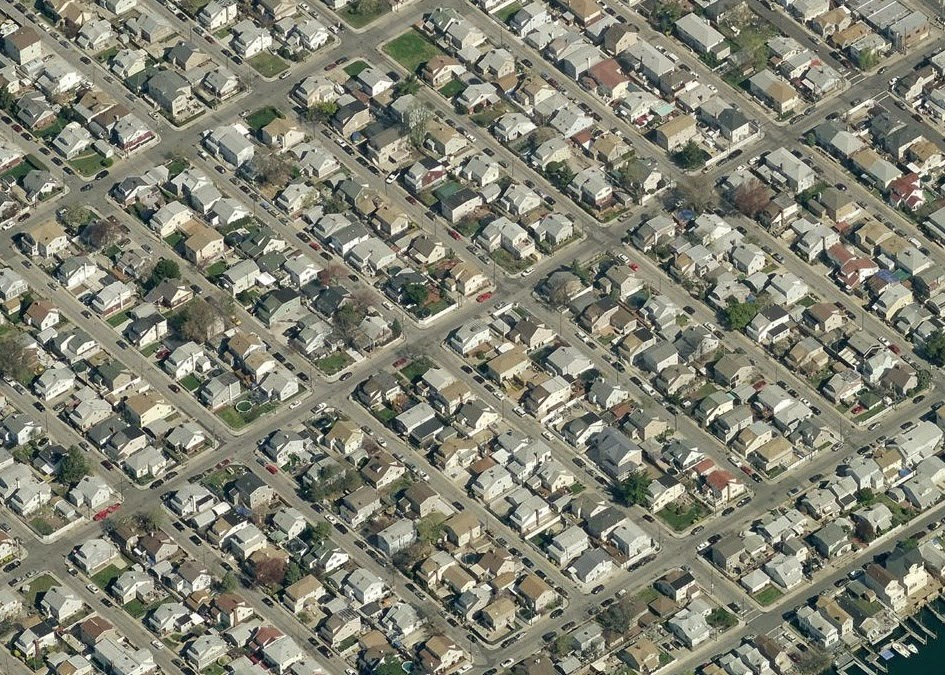
\includegraphics[width = \textwidth]{Gerritsen.jpg}
\end{frame}
\addtocounter{framenumber}{-1}


\begin{frame}{Motivation}
	\begin{itemize}
		\itemsep1em
		\color{black}
\item Pervasive US Housing regulation is playing a role in housing unaffordability, with real consequences for \color{red} aggregate growth \color{black} \citep{hseihmoretti} \citep{durantonpugaurbgrowth} \citep{parkho} \pause

\item Lot size regulation disproportionately burdens low income families, causing considerable \color{red} residential sorting on income \color{black} and race  \citep{kulka} \citep{Song}. \pause

\item How does the minimum lot size shape \textit{aggregate welfare} and \textit{urban structure}?
\begin{itemize}
	\item The sizes of productive cities? \dots 
	\item The location of affluent neighborhoods in those cities?
\end{itemize}


	\end{itemize}
\end{frame}


\begin{frame}{In this paper}
	\begin{enumerate}
		\itemsep1em
		\color{black}
		\item Income sorting has important implications for the \textit{aggregate} welfare consequences of regulation, building on \cite{hseihmoretti} and \cite{durantonpugaurbgrowth}:
		\begin{itemize}
			\item Deregulation causes high income, productive households to sort out of productive cities
			\item Exacerbated when local amenities are endogenous
			\item Ensuing externalities, e.g. \cite{hamilton1976}. 
		\end{itemize} \pause
		\item  Evidence that \textit{heterogeneous} regulation has altered the urban structure of expensive cities. Within city migration is crucial for assessing welfare consequences in the model:
		\begin{itemize}
		\item Evidence that low income households choose high density neighborhoods to avoid stringent lot sizes
		
		\item This choice imposes externalities through the endogenous supply of amenities
		\end{itemize}
	\end{enumerate} 
\end{frame}

\begin{frame}{How?}
	\begin{itemize}
		\color{black}
		\itemsep1em
		\item Build and calibrate a structural GE model with heterogenous households, cities and neighborhoods across the contiguous United States
		\begin{itemize}
			\color{black}
			\itemsep1em
			\item (Heterogenous) regulations cause income sorting both \color{red} within \color{black} and  \color{red} across \color{black} cities \dots
			\item and income sorting endogenously shapes the pattern of neighborhood amenities 
		\end{itemize}
	\pause
		\item Focus on a simple counterfactual:
		\begin{itemize}
			\itemsep1em
			\color{black}
			\item Removing all measured lot size restrictions across MSA's within the contiguous United States \pause
			\item Ignores the political economy of housing regulation, unlike \cite{parkho} or \cite{bunten}  
		\end{itemize}
	\end{itemize}
\end{frame}

\begin{frame}{Preliminary Results: Welfare}
	\begin{itemize}
		\color{black}
		\itemsep1em
		\pause
		\item Substantial welfare gains across the board
		\begin{enumerate}
			\itemsep1em
			\item \textit{Average} household gains approximately $10.2 \%$. \\ These gains are extremely skewed toward low income households ($< \$25,000$ yearly). \pause
			
			
			\item \textit{Average} landlord sees their land values rise by $5 \%$. \\
			However, strongly regulated neighborhoods lose substantially, and this is driven entirely by endogenous amenities. 
		\end{enumerate} \pause
		
		
		\item The endogenous supply of amenities account for approximately \textit{half} of these gains to households of \textit{all} income groups.
		\begin{itemize}
			\item Inuition: Many high income households live \textit{outside} of neighborhoods with large lots in the data.
			\item They \textit{benefit} from the movement of low income households after deregulation!
		\end{itemize}
	\end{itemize}
\end{frame}		
		
	\begin{frame}{Preliminary Results: Urban Structure}
		\begin{itemize}
			\color{black}
			\itemsep1em
		\item Counterfactual equilibrium hints at the importance of within \textit{and} across city sorting for welfare 
		
		\item \color{purple} Across \color{black} cities: \cite{hseihmoretti} style productivity gains are \color{red} completely nullified \color{black} by the \color{red} weakening \color{black} of income sorting into expensive cities.
			
		\item \color{purple} Within \color{black} cities: a \color{red} weakening \color{black} of \color{red} negative income sorting \color{black} into the high density neighborhoods of expensive cities.
		\begin{itemize}
			\itemsep1em
			\item \textit{Gentrification accelerates}, and the affluent households who locate in these neighborhoods benefit from it.
		\end{itemize}
	\end{itemize}
\end{frame}


\begin{frame}{Estimation}
\begin{itemize}
	\itemsep1em
	\color{black}
	\item Housing regulation is hard to measure, but recent advances...
	\begin{itemize}
		\item \cite{Song} shows that a structural break detection algorithm works well for minimum lot sizes
		
		\item I adapt a variation of this procedure using assessment data
	\end{itemize}

	\item Endogenous amenities $\implies$ key identification challenge
	\begin{itemize}
		\item Employ a lot-level "donut design" following \cite{kulka}, \cite{anagoletal2021}, and originally \cite{BFMJPE}
		\item Use terrain slopes as an IV 
		\item This still needs to be completed
		\item For this draft I use an identification strategy from my previous presentation 
	\end{itemize}
\end{itemize}	
\end{frame}

	\begin{frame}{Literature}
		\fontsize{8pt}{7.2}	
		\begin{itemize}
			\itemsep1em		
			
			\item \color{red} Macroeconomics of housing regulation \citep{hseihmoretti} \citep{durantonpugaurbgrowth} \citep{parkho} \citep{bunten} \citep{hop} \citep{ganongshoag} \citep{superstarcities} 
			
			
			\item \color{red} Lot Size/Unit density regulation \citep{kulka} \citep{Song} \citep{KSC} \citep{zabel} \citep{gyourko2021} \citep{griesonwhite} \citep{gyourkovoith1997} \citep{davidoff2022}
			
			\item \color{red} Housing Regulation + Supply + Affordability \citep{BSH} \citep{saiz2010} \citep{asquithetallocaleffects} \citep{mastwarding} \citep{albouyetal} \citep{bbheight} \citep{mills2005} \citep{bruecknersingh} \citep{BruecknerFuGu} \citep{acosta} \citep{martynov} \citep{turner2014} \citep{gyourkomolloy} \cite{anagoletal2021}
			
			\item \color{purple} Urban spatial sorting \citep{diamond2016} \citep{couturehandbury} \citep{su2021} \citep{bshartley2020} \citep{Coutureetal} \citep{AlmagroDI} \citep{parispoor} \citep{ccpoortransport} \citep{Gentrificationcycles} \cite{LeeandLin}
			
			\item \color{purple} Inequality in cities \citep{ineqcitysize} \citep{spatialsorting} \citep{FogliGuerrieri}
			
			\item \color{teal} Exclusionary Zoning \citep{Hamilton1975} \citep{calabresetal} \citep{keepingpeopleout} \citep{ineffTiebout} \citep{barcoate} \citep{brueckner2021}
		\end{itemize}
	\end{frame}

\section{Motivating Evidence}

\begin{frame}{Fact 1: Strong Income Sorting on Density in Expensive Cities}
\begin{itemize}
	\itemsep1em
	\color{black} \pause
	\item Using block-group level data from the 2008-2012 ACS \pause
	\item Within each 2013 MSA, I rank block groups by their density of housing units. Ranking lies in the unit interval. \pause
	\item I flexibly regress (log) average income against this ranking separately for both the "Superstar" and "Non-Superstar" samples. \pause
	\item Superstars are MSAs in the top quartile of (unadjusted) housing prices, Non-superstars in the bottom quartile \pause
	\item log Average income is demeaned by MSA to control for fixed effects.
\end{itemize}
\end{frame}

\begin{frame}{Fact 1: Strong Income Sorting on Density in Expensive Cities}\label{Fact1}
	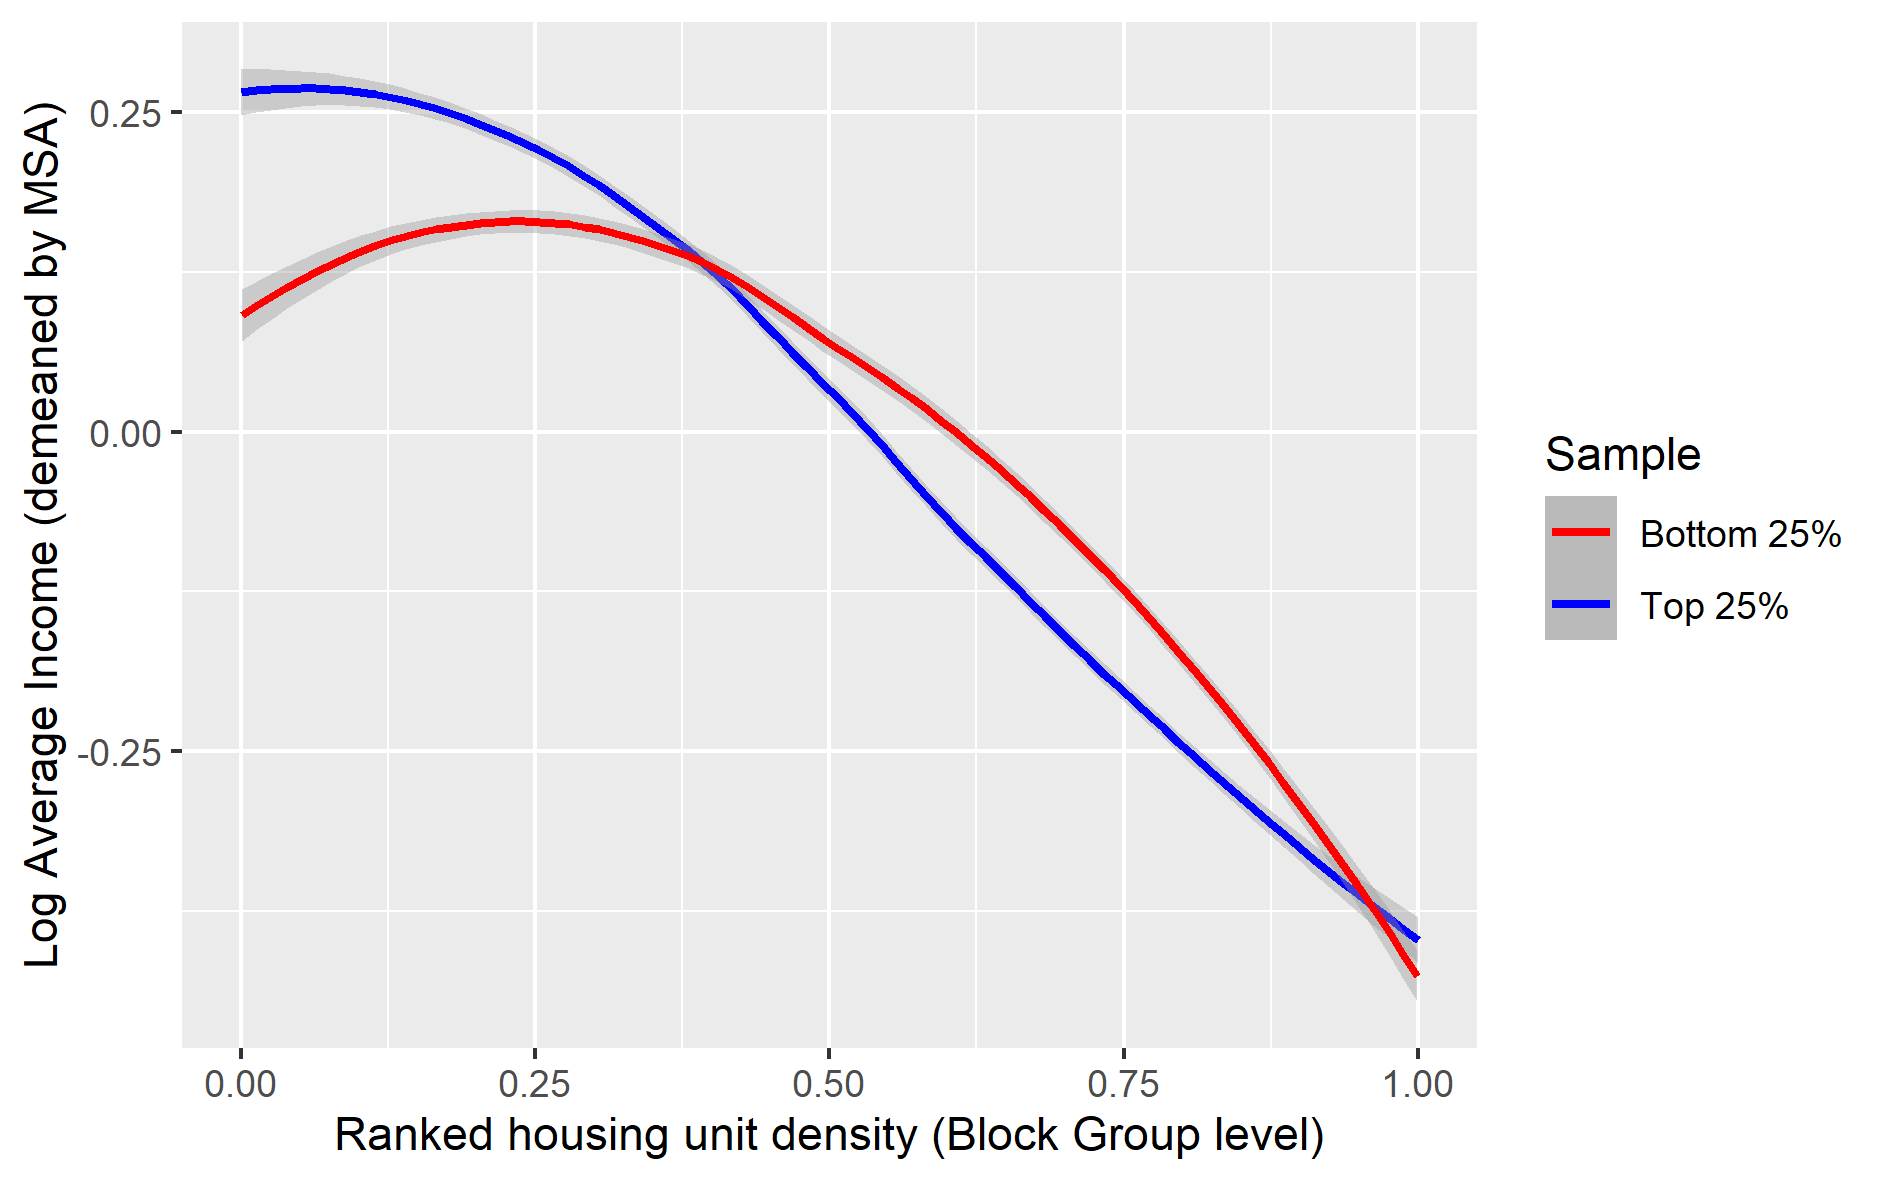
\includegraphics[width= \textwidth]{income.png}
	\hyperlink{Ctfl_Income_gradient}{\beamerbutton{Counterfactual}} 
\end{frame}

\begin{frame}{Fact 2: Patterns of Lot Size Stringency}
	\begin{itemize}
		\color{black}
		\itemsep1em
		\item Can we link these income sorting patterns to \textit{direct} measures of lot size stringency?
		\pause
		\item Model yields a simple statistic $\mathbb{I}^{\star}(i)$: \textit{the cost to rent structure on a lot at the minimum size} in block group $i$.
		\begin{equation}
			\mathbb{I}^{\star}(i) = V(i)l(i)
		\end{equation}
		\begin{itemize}
			\itemsep1em
			\color{black}
			\item Assuming we \color{red} observe \color{black} the minimum lot size $l(i)$ (in acres) and value of housing per acre $V(i)$ 
			\item \dots and that they are uniform within the block group 
		\end{itemize}
	\pause
	\item Constructed from most recent assessment data as of 2015
	\end{itemize}
\end{frame}

\begin{frame}{Fact 2: Patterns of Lot Size Stringency}
		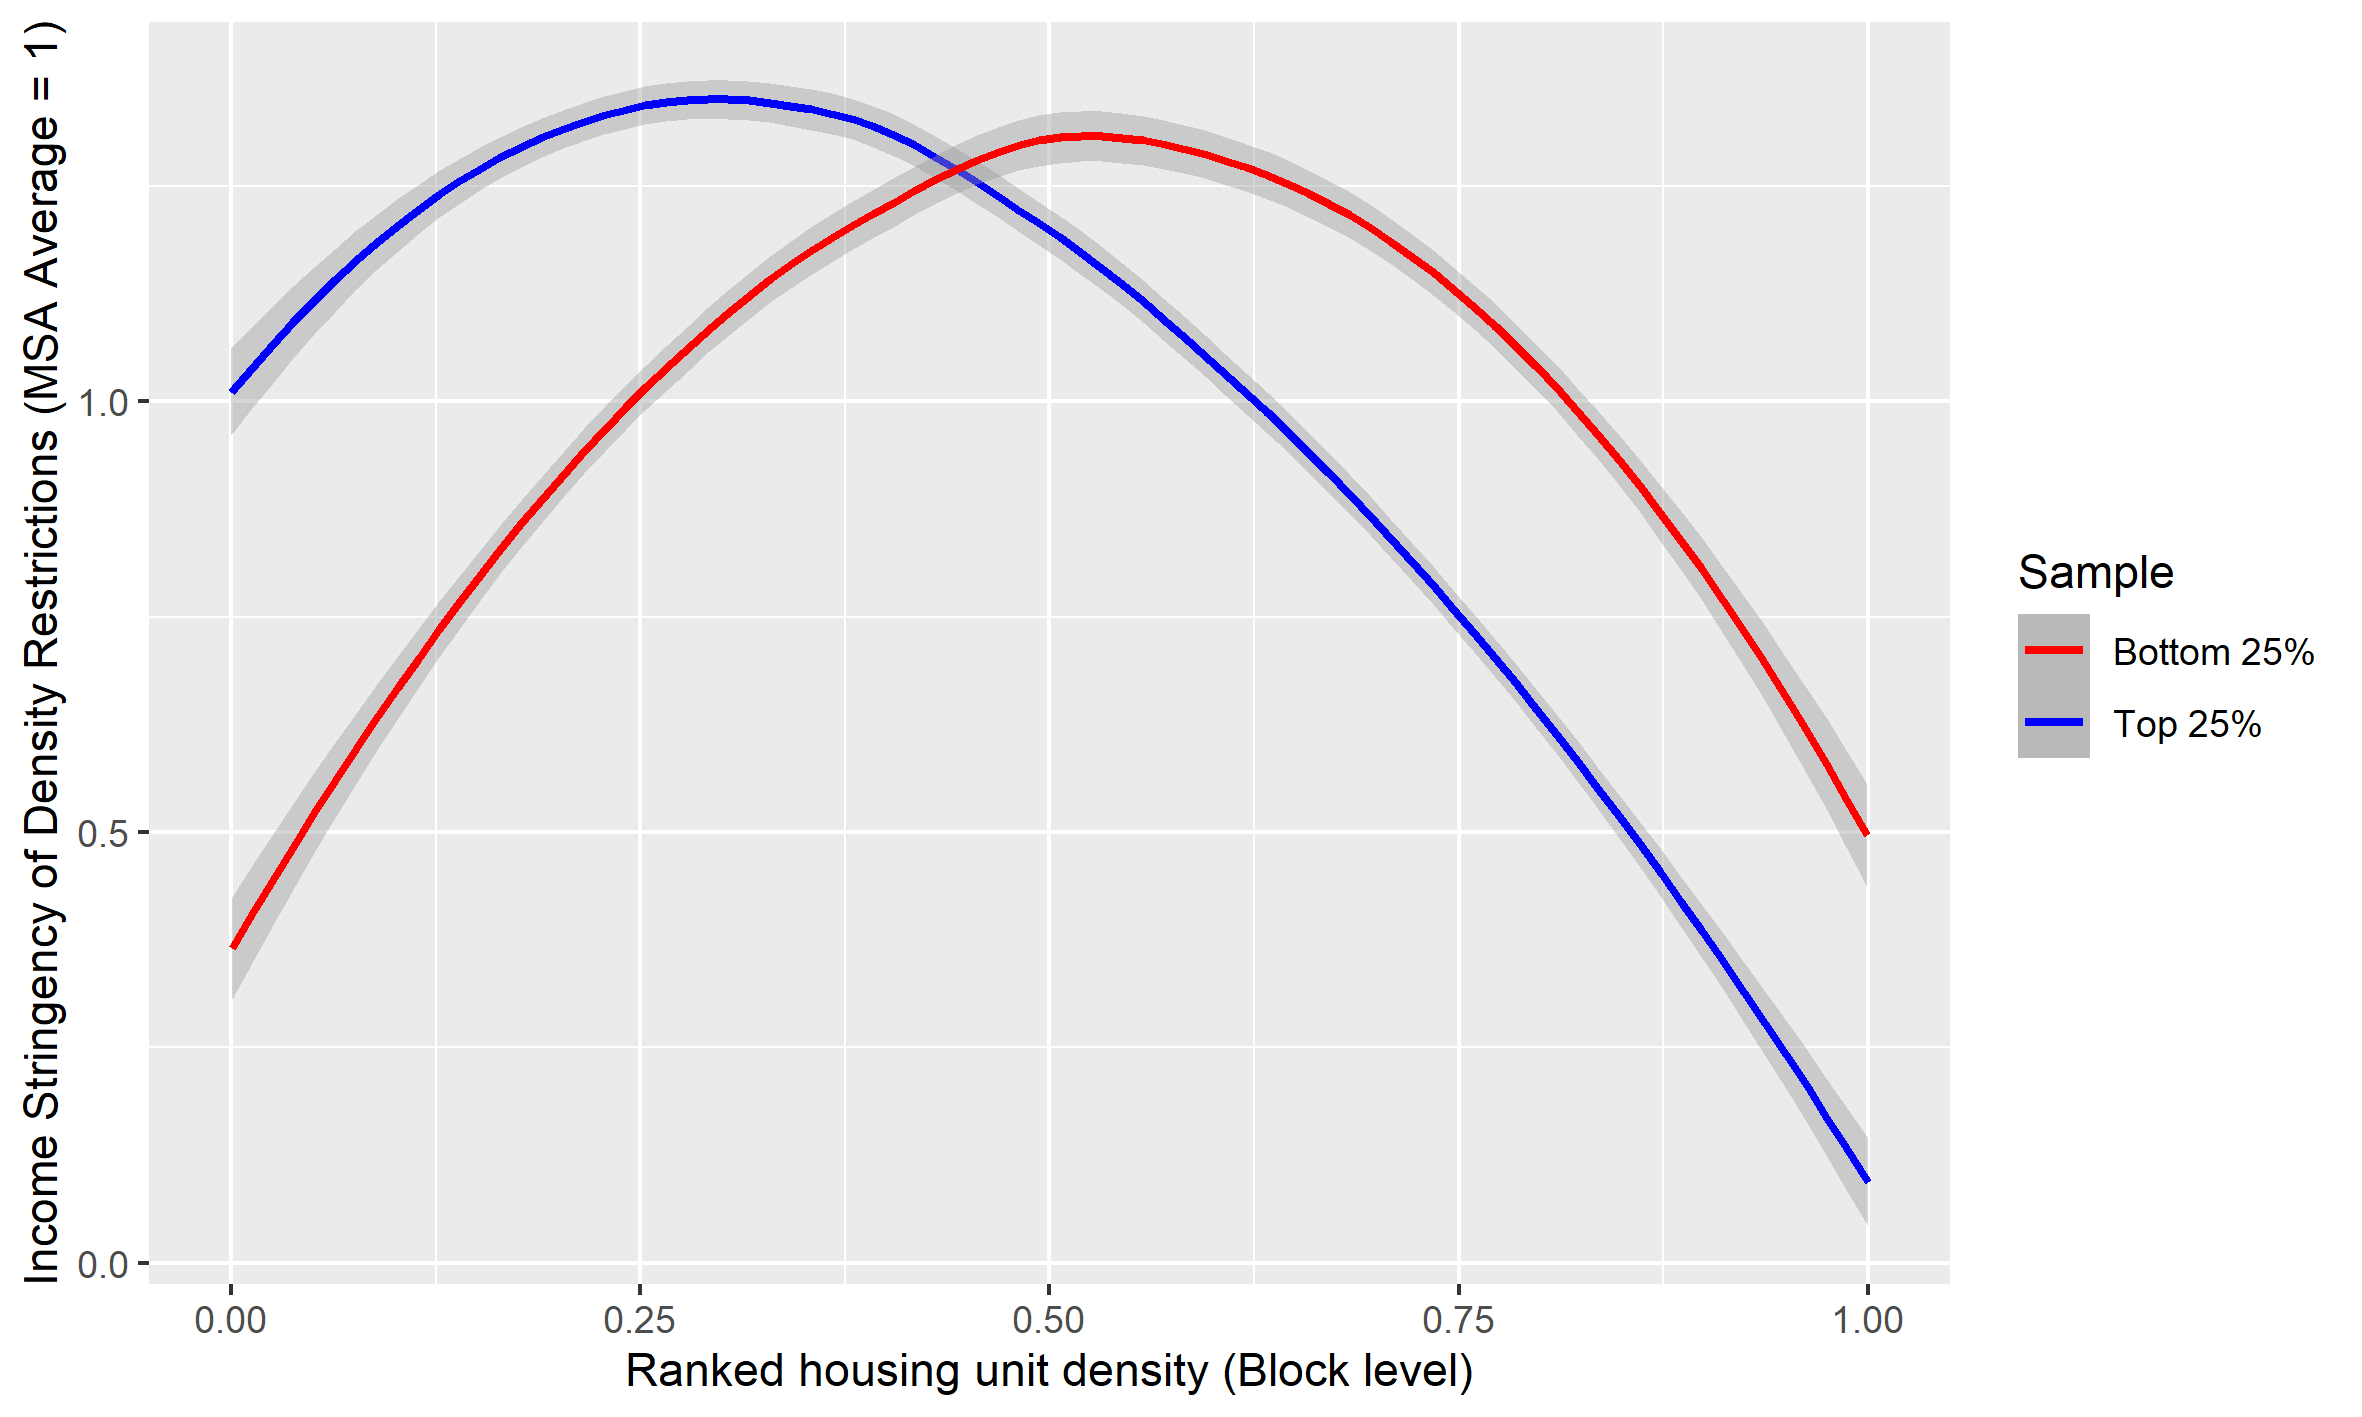
\includegraphics[width= \textwidth]{stringencyofDensityRestrictions.png}
\end{frame}

\section{Model}

\begin{frame}{Preliminaries}
	\begin{itemize}
		\color{black}
		\itemsep1em
		\item Let $i$ index a particular 2010 block group; will be the definition of a \textit{neighborhood} in the model.  \pause
		
		\item Let $C(i)$ be the 2013 MSA associated with $i$ \pause
		
		\item Let $N(c)$ be the set of neighborhoods contained in MSA $c$ \pause
		
		\item Unless otherwise stated, all data are from the 2010 Census or the 2008-2012 ACS, where applicable. \pause
		
		\item Each block group $i$ has land $T_{R}(i)$ available for residential  development.  
	\end{itemize}
\end{frame}


\begin{frame}{Developer's Problem}
	\begin{itemize}
		\color{black}
		\item Start with a standard Cobb-Douglas production function for housing, yielding housing supply per unit of land
		\begin{equation}
			A(i) = \lambda(i)P(i)^{\epsilon(i)}
		\end{equation} \pause
		
		
		\item Minimum lot sizes complicate things. Developers need to \color{red}\textit{respect the allocation of housing stock across housing units}\color{black}.
		
		\item Minimum lot sizes $l(i)$ incentivize developers to build above a \textit{minimum housing stock per housing unit}   \pause
		\begin{equation}
			A^{\star}(i) = \lambda(i)P(i)^{\epsilon(i)}l(i)
		\end{equation} \pause
		\item Define: $\mathbb{I}^{\star}(i) := P(i)A^{\star}(i)$, which is increasing in $P(i)$ and $l(i)$
	\end{itemize}
\end{frame}

\begin{frame}{Consumer's Problem}
	\begin{itemize}
		\color{black}
		\itemsep1em
		\item Suppose a household chose neighborhood $i$ in city $C(i)$: \pause
		\item Households differ on effective units of labour $f \in F$ and education $s$, receive a city-education specific wage $w_{s}(c)$ \pause
		\item Household has Cobb Douglas preferences over housing $A$ and numeraire good $g$
		\begin{equation}\label{utility}
			\max_{A, g} A^{\beta}g^{1-\beta}
		\end{equation} 
		subject to \color{red}$P(i)A \geq \mathbb{I}^{\star}(i)$ \color{black} and $P(i)A + g \leq w_{s}(i)f$. \pause
		
		\item Let $z$ index both education and units of labour, and let $V(i, z)$ be the indirect utility associated with this problem. \pause 
		
		\item Features \textit{income sorting}: $\frac{\partial}{\partial f}\bigg[-\frac{\partial V(i, z)}{\partial \mathbb{I}^{\star}(i)}\bigg] \leq 0 $ 
	\end{itemize}
	
\end{frame}

\begin{frame}{Neighborhood Choice}
	\begin{itemize}
		\color{black}
		\item Households receive \textit{type-specific} amenity $b(i, z)$ \pause
		\item Gumbel shocks over neighborhoods with nests across and within cities. Labour supply for type $z$ households are 
		\begin{equation}\label{laboursupply}
	L(i, z) = \bigg[\frac{e^{\theta(z) W(C(i), z)}}{e^{\boldsymbol{W}(z)}}\bigg]\bigg[\frac{b(i, z)e^{\rho(z) V(i, z)}}{e^{W(C(i), z)}}\bigg]\bar{L}(z)
		\end{equation}
		\pause with 
		\begin{equation*}
 	W(C(i), z) = \log\bigg[\sum_{i' \in N(C(i))}b(i', z)e^{\rho(z) V(i', z)}\bigg]
		\end{equation*} 
		\pause and
		\begin{equation*}
\boldsymbol{W}(z) = \log\bigg[\sum_{c \in C} e^{\theta(z) W(c, z)}\bigg]
		\end{equation*}
	\end{itemize}
\end{frame}

\begin{frame}{Endogenous Amenities}
	\begin{itemize}
		\color{black}
		\itemsep1em
		\item  Let $\tau(i)$ be the commuting time in $i$. I allow amenity values $b(i, z)$ to respond to neighborhood income per capita via the equation:
		\begin{equation}
			\log\big[b(i, z)\big] = -\kappa\tau(i) + \Omega\log\bigg[AverageIncome(i)\bigg] + \epsilon(i, z)
		\end{equation} \pause
		\item Two microfoundations 
		\begin{enumerate}
			\itemsep1em
			\item Local, non-traded Dixit-Stiglitz market  \citep{Coutureetal} \citep{AlmagroDI} + local disutility of density \citep{KSC} \pause
			\item Local, congested public good financed through property taxes \citep{calabresetal} \citep{ineffTiebout}
		\end{enumerate}
	\end{itemize}
\end{frame}

\section{Calibration + Identification}

\begin{frame}{Measuring Minimum Lot Sizes}\label{returnZoningDist}
	\begin{itemize}
		\color{black}
		\itemsep1em
		\item Follows a structural break algorithm in \cite{Song}.
		\begin{itemize}
			\item Idea: Zoning variances are present, but rare 
			\item Implies "bunching" of lot sizes around the minimum, which can be fit with a discontinuous CDF  \pause 
			\item Problem: Need sufficient amount of data within "zoning districts" to rule out \textit{spurious discontinuities}
			
		\end{itemize} \pause
		
		\item How would one construct these "Zoning Districts"?
		\begin{itemize}
			\item Clustering algorithm of \cite{Chavent2018}
			\item Cluster on shares of single family/multifamily homes + modes and quartiles of their lot size distributions; commercial and vacant land shares
			\item allows one to weigh the importance of geographic proximity in assigning clusters
		\end{itemize}
	\item Clusters approx. 174,000 block groups into 20,000 Zoning Districts 	\hyperlink{zoning}{\beamerbutton{Zoning Districts}} 
	\end{itemize}
\end{frame}

\begin{frame}{Measuring Minimum Lot Sizes}\label{returnLotSize}
	\begin{itemize}
		\itemsep1em
		\color{black}
		\item Take the (smallest) mode of the lot size distribution \pause
		
		\item I generalize this procedure to multifamily structures (duplexes, triplexes and fourplexes) by re-scaling by the implied unit density restriction 
		\begin{itemize}
		\item Allow for multifamily structures in $i$ if fraction of corresponding housing units (from ACS) exceed $35 \%$ 
		\end{itemize}	
			\pause
		
		\item Additional cleaning:
		\begin{itemize}
			\item Remove regulation if $35 \% $ of lots below measured minimum
			\item Remove regulation if the implied number of housing units at the measured lot size exceeds measure of residential land use $T_{R}(i)$
			\item Top-coding at 5 acres (only 400 block groups are changed)
		
		\end{itemize}	
	
	
	\hyperlink{lotsizecdf}{\beamerbutton{Measurements}} 
	\end{itemize}
\end{frame}

\begin{frame}{Prices, Wages, and Other Parameters}
	\begin{itemize}
		\color{black}
		\item Prices $P(i)$ 
		\begin{itemize}
			\item Hedonic regression following \cite{BSH} using characteristics from assessments
		\end{itemize}\pause
		
		\item Wages $w_{s}(c)$
		\begin{itemize}
			\item Mincer style regression with city fixed effects, following \cite{ineqincreased}
		\end{itemize} \pause
		 
		\item $\beta$ and supply shifters $\lambda(i)$
		\begin{itemize}
			\item $\beta$ chosen to target spending share of 0.2 \citep{orlatomagnedavis}
			\item $\lambda(i)$ chosen to clear housing markets at prices $P(i)$ under implied spending
		\end{itemize} \pause
	\item Migration Elasticities + Amenities $b(i, z)$
	\begin{itemize}
		\item Rescale $\theta(z)$ and $\rho(z)$ to match migration elasticity estimates from \cite{morettihornbeck} across cities and \cite{herzog2022} within cities. \pause
		
		\item $b(i, z)$ chosen to rationalize $L(i, z)$ after appropriate choice of support of $Z$. 
	\end{itemize}
	\end{itemize}
\end{frame}

\begin{frame}{Estimating $\Omega$}
		\begin{itemize}
		\color{black}
		\itemsep1em
		\item Recall the estimating equation: 
		\begin{equation*}
			\log\big[b(i, z)\big] = -\kappa\tau(i) + \color{red} \Omega \color{black} \log\bigg[AverageIncome(i)\bigg] + \epsilon(i, z)
		\end{equation*} \pause
		\item Identification challenged by a  \textit{simultaneity bias} analogous to \cite{diamond2016} or \cite{LeeandLin}.
		\begin{itemize}
			\item Reverse Causality -- unobserved neighborhood demand shocks $\epsilon(i, z)$ \color{red} exacerbate income sorting \pause
		\end{itemize} 
	 \item Sloped terrain does well at \textit{predicting} income per capita \citep{saiz2010} 
	 \begin{itemize}
	 	\item One problem: they enter directly into the demand for neighborhoods.
	 \end{itemize}
	\end{itemize}
\end{frame}

\begin{frame}{Estimating $\Omega$}
	\begin{itemize}			\color{black}	\itemsep1em
	\item Propose a "donut" style instrument \citep{BFMJPE}
	\begin{itemize}
	\itemsep1em
		\item For some house $h$, use the slopes of houses within some distance $d$ from the lot as an instrument for income per capita of neighbors
		
		\item \textit{This is after controlling for slopes very close to the lot of house $h$}.
		 
		\item Disaggregate choice model to the house level \color{red} for estimation only. \color{black} 
	\end{itemize} \pause
	\item Identification assumptions: 
	\begin{enumerate}
		\item Amenity value of sloped terrain  \textit{decays completely at distance $d$ from the lot}.
		\item Sloped terrain of neighbors at distance $d$ uncorrelated with other demand factors conditional on own slopes. 
	\end{enumerate} \pause
	\item For this draft: $\hat{\Omega} = 2.65$ estimated using a tract-level strategy from my previous presentation.
\end{itemize}
\end{frame}

\section{Counterfactual Results}

\begin{frame}{The sources of welfare gains}
	\begin{itemize}
		\color{black}
		\itemsep1em
		\item Focus on a simple counterfactual -- setting $l(i) = 0$ in all neighborhoods. \pause
		
		\item 4 channels in which deregulation affects welfare:
		\begin{enumerate}
			\itemsep1em
			\item Households can purchase smaller lots below (binding) minimum lot size
			\item Gains from the expansion of productive cities \citep{hseihmoretti}
			\item Correcting inefficiencies caused by altering urban structure, such as inefficient sprawl or density \citep{bbheight}
			\item Endogenous amenities 
		\end{enumerate}
	\end{itemize}
\end{frame}


\begin{frame}{Welfare By Household Type}\label{returnWelfare}
		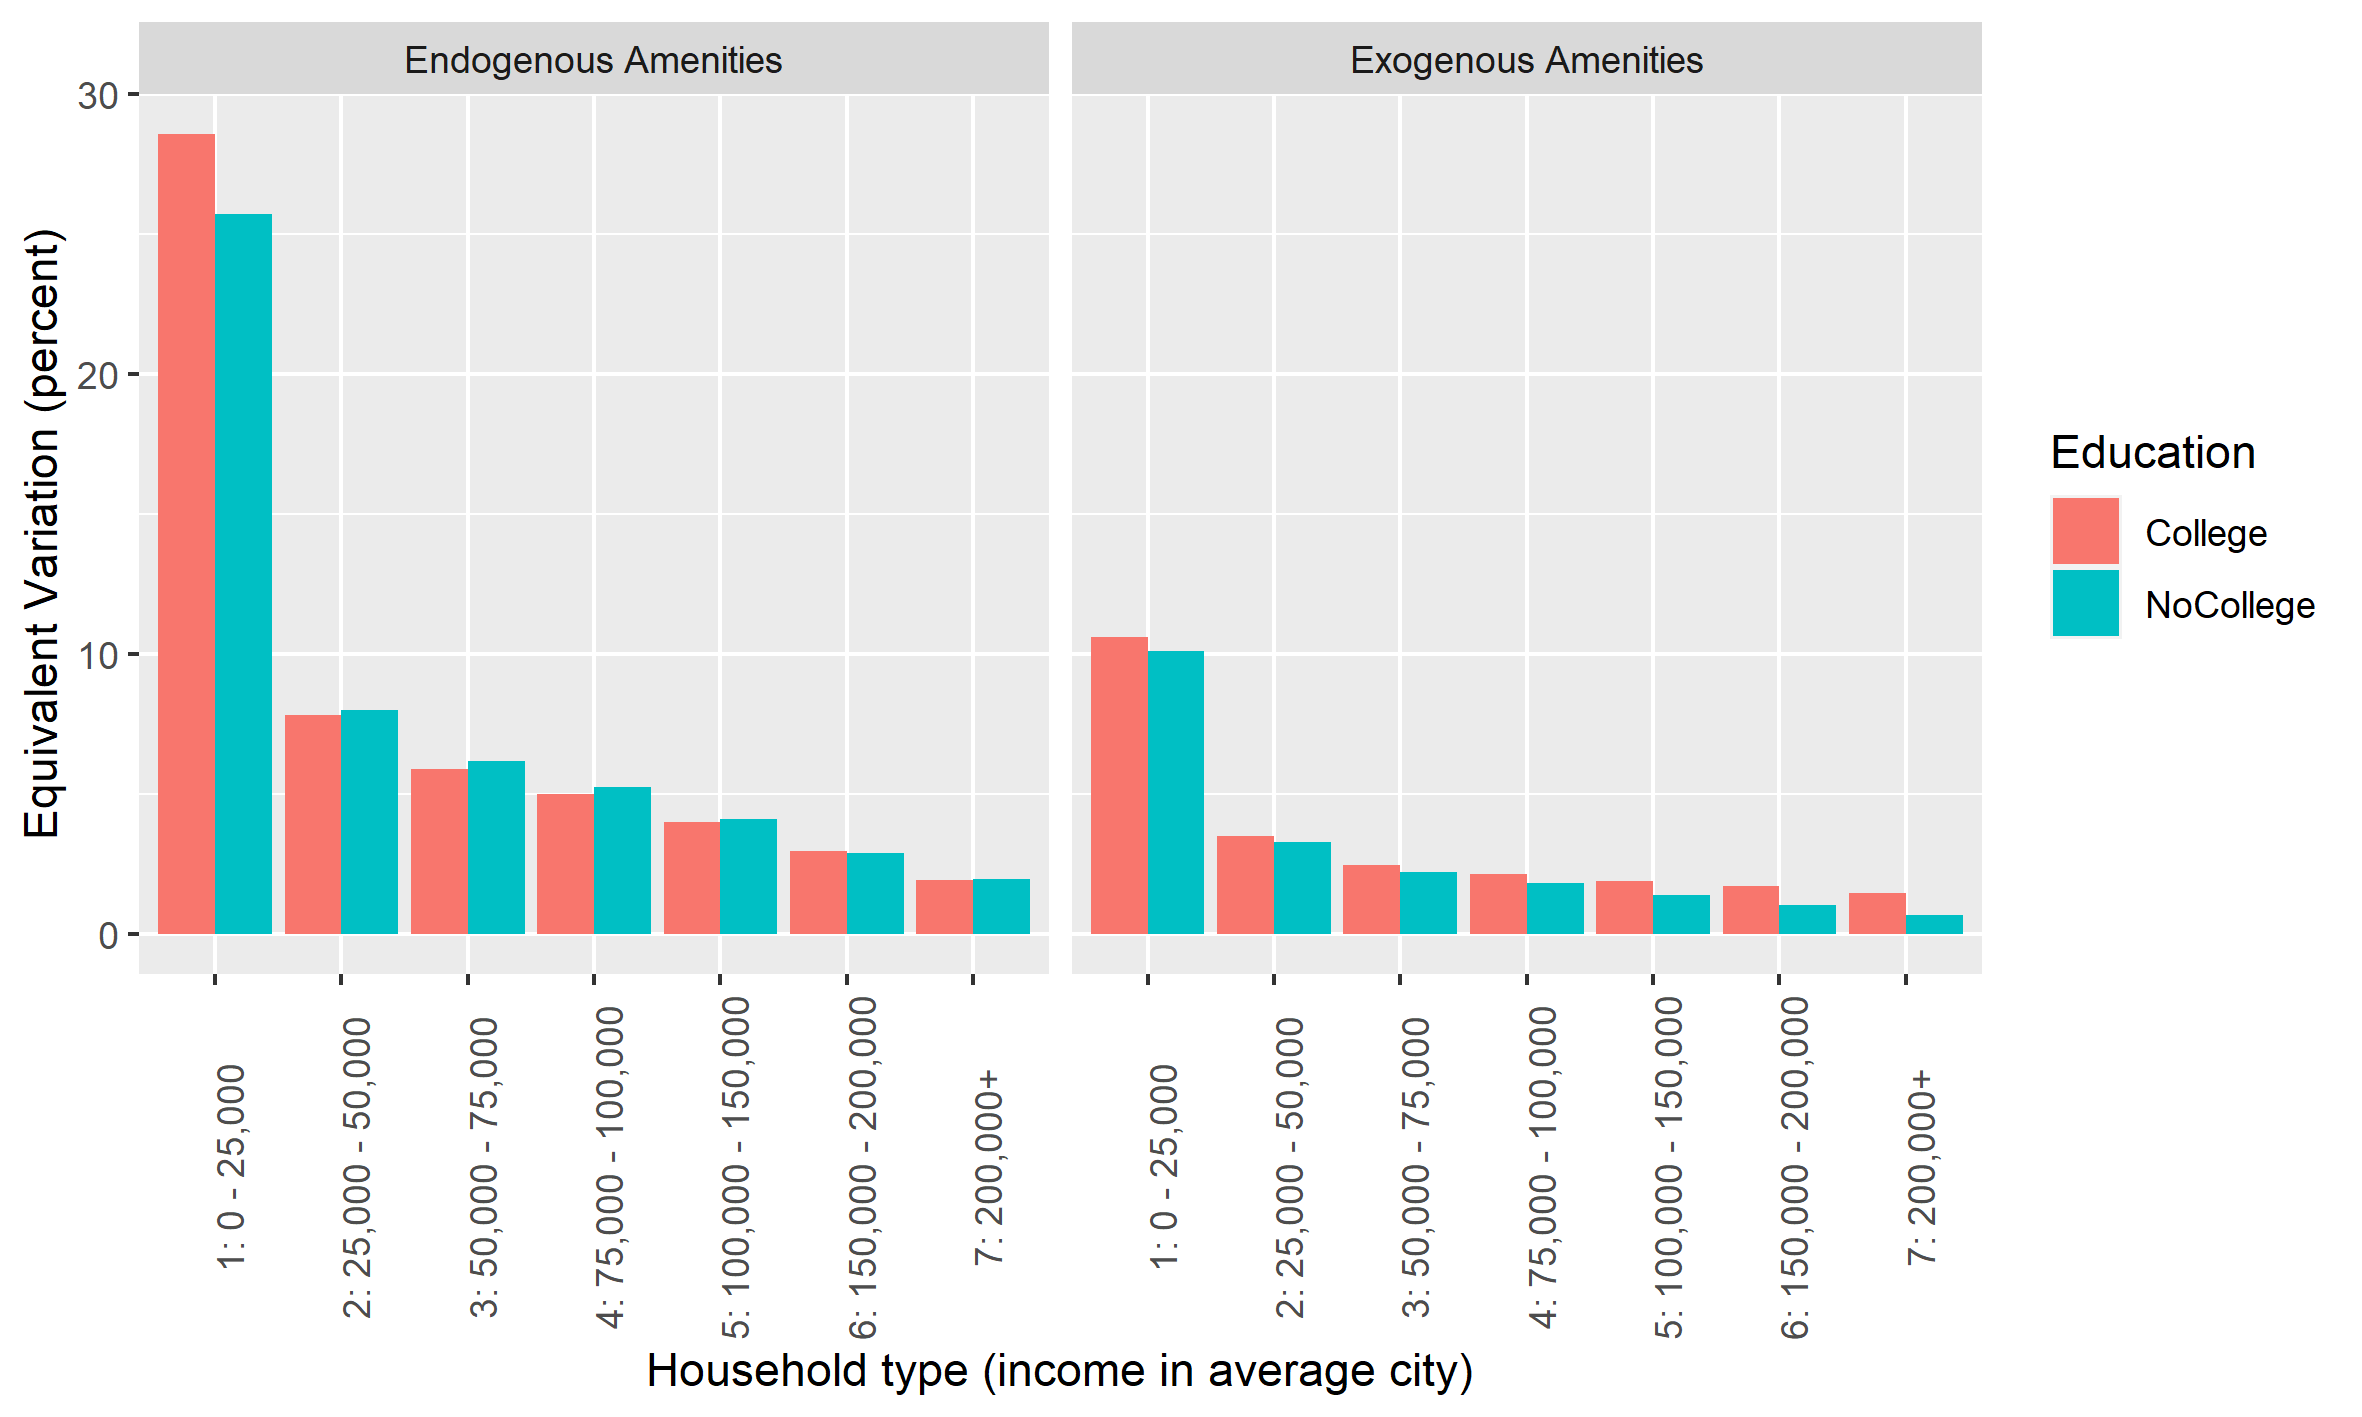
\includegraphics[width=\textwidth]{Welfare.png}

	\hyperlink{intuition}{\beamerbutton{Framework?}} 
\end{frame}

\begin{frame}{No Labour Productivity Gains}
	\pause
	\begin{figure}[htbp]
	\centering
	
	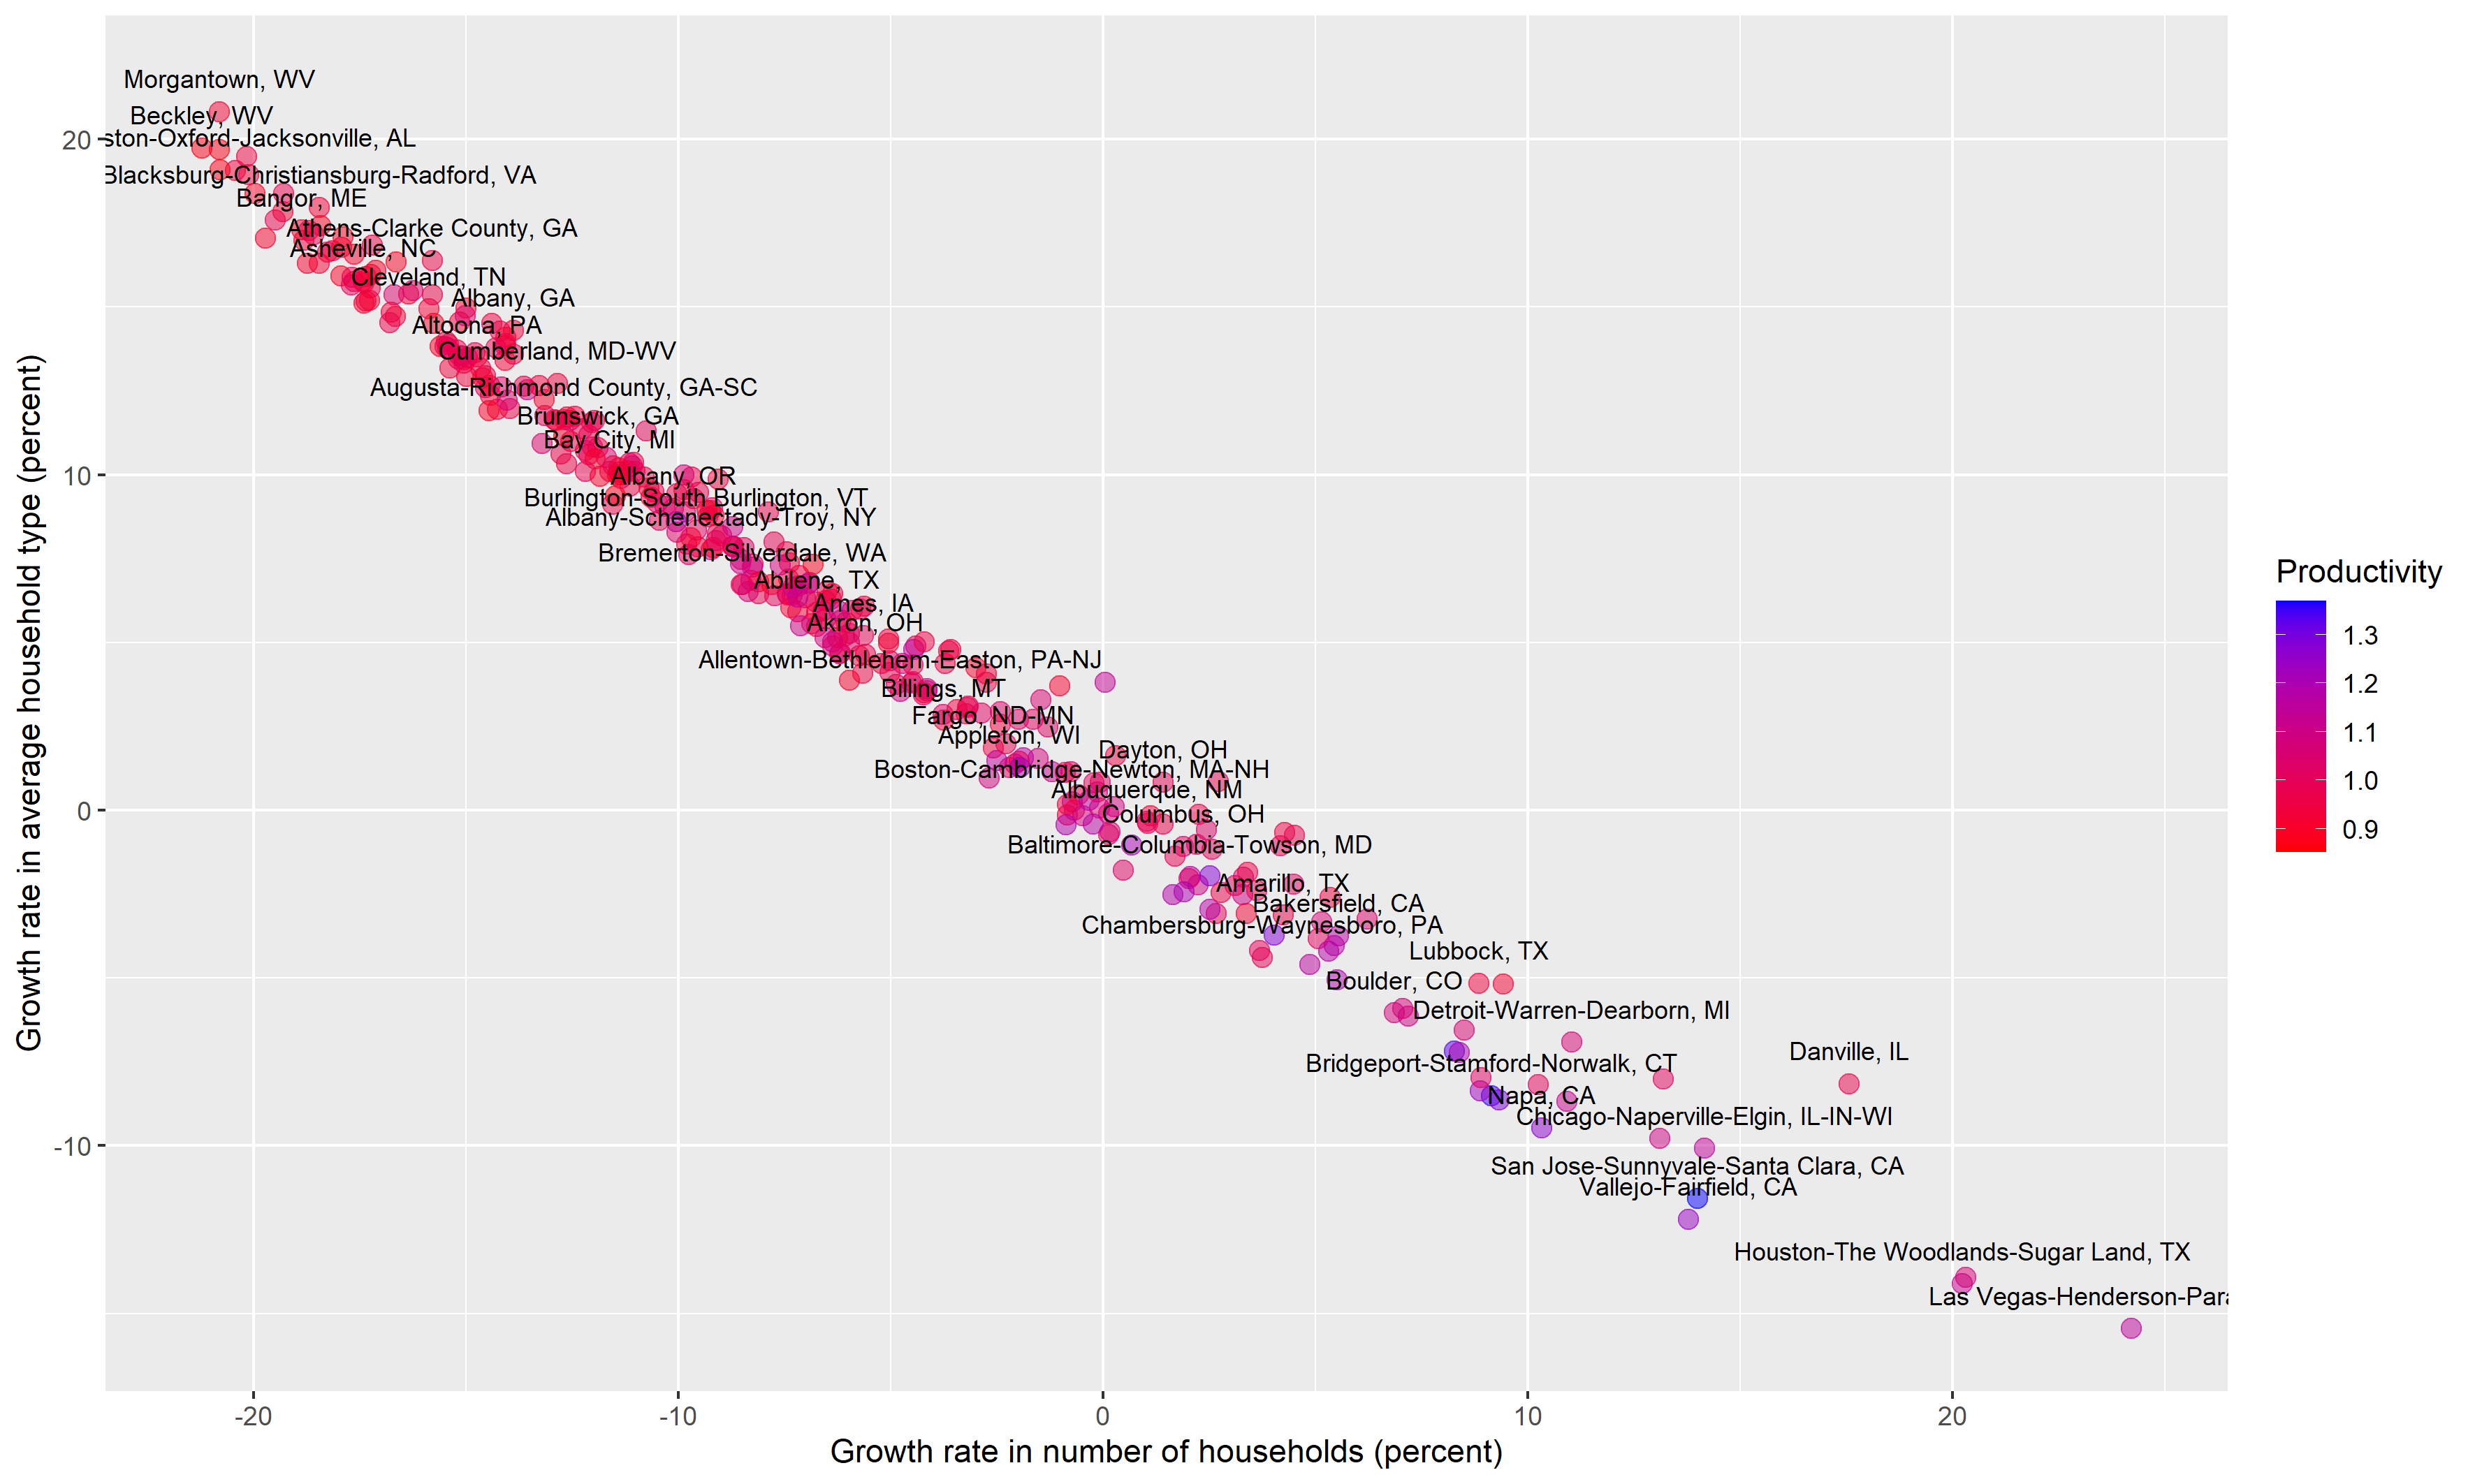
\includegraphics[width=\textwidth]{IncomeSortingMovement.png}
	
	\caption*{\scriptsize The y axis is defined as the change in the average income that a household could earn in an average city. Productivity is defined as the average of the college and non-college wages per unit of labor. Correlation between growth rate in the number of households and productivity is approximately 0.55.}
	
\end{figure}
\end{frame}

\begin{frame}{Welfare of Landlords in previously regulated neighborhoods}
	\pause
	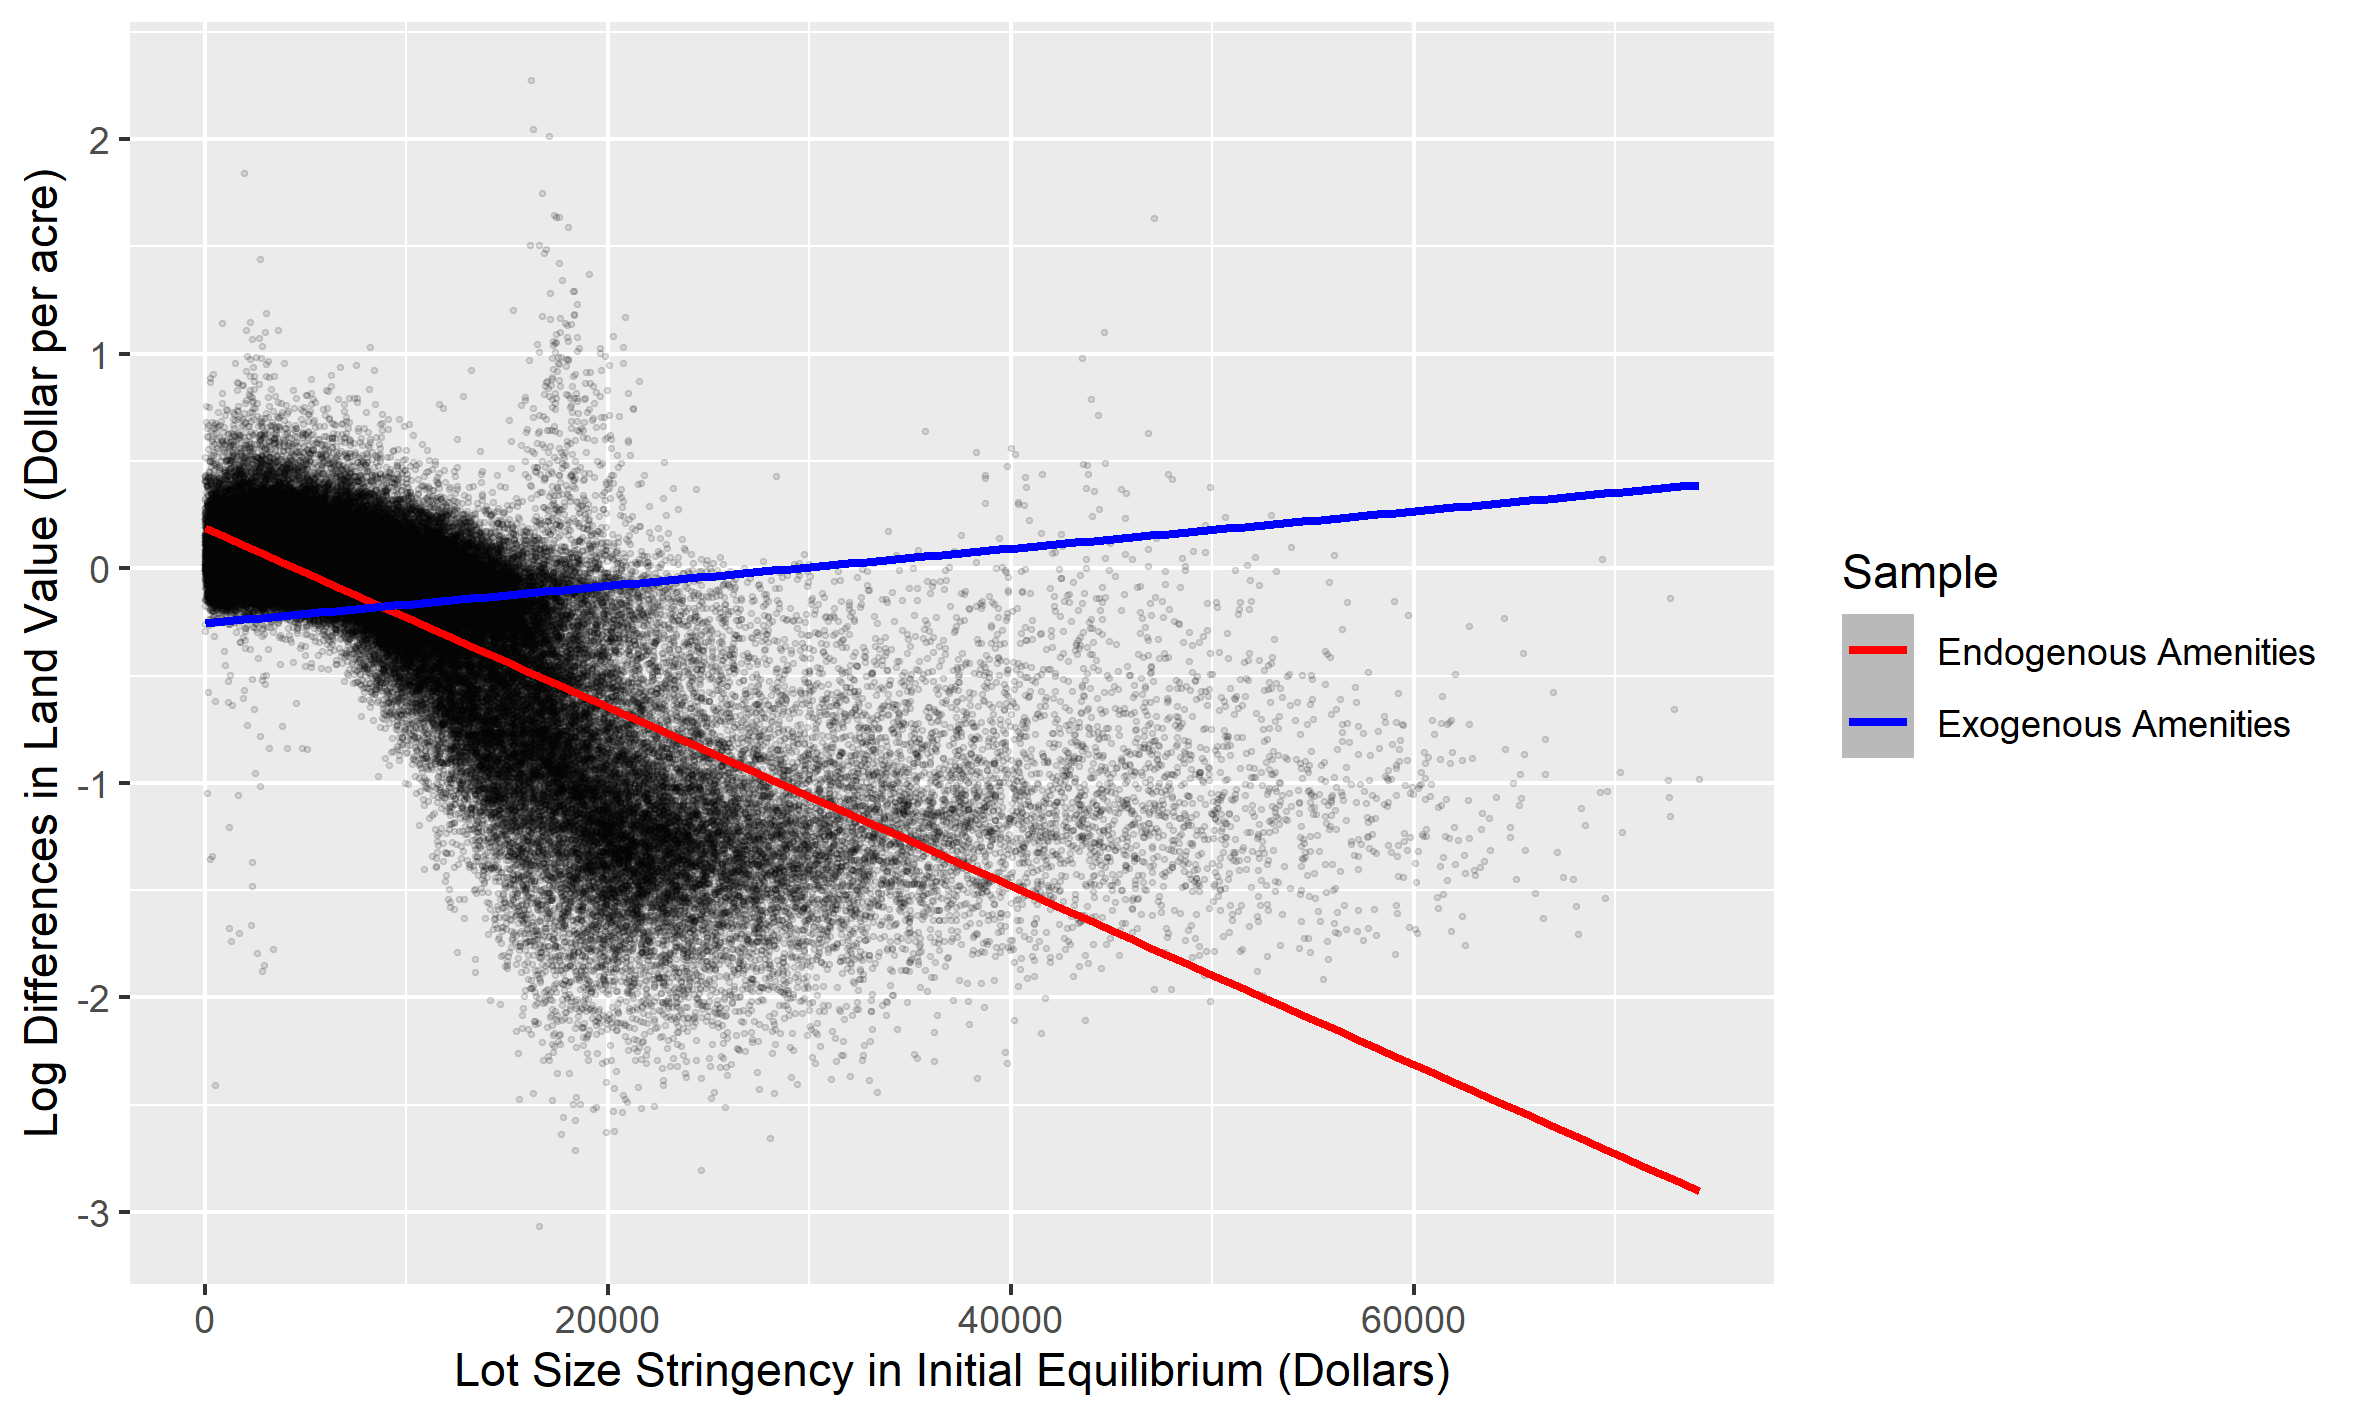
\includegraphics[width = \textwidth]{StringencyChangeLandVal.png}
	\begin{itemize}
		\item Note: x axis is just the $\mathbb{I}^{\star}(i)$ in the model. 
	\end{itemize}
\end{frame}


\begin{frame}{Counterfactual income gradients}\label{Ctfl_Income_gradient}
		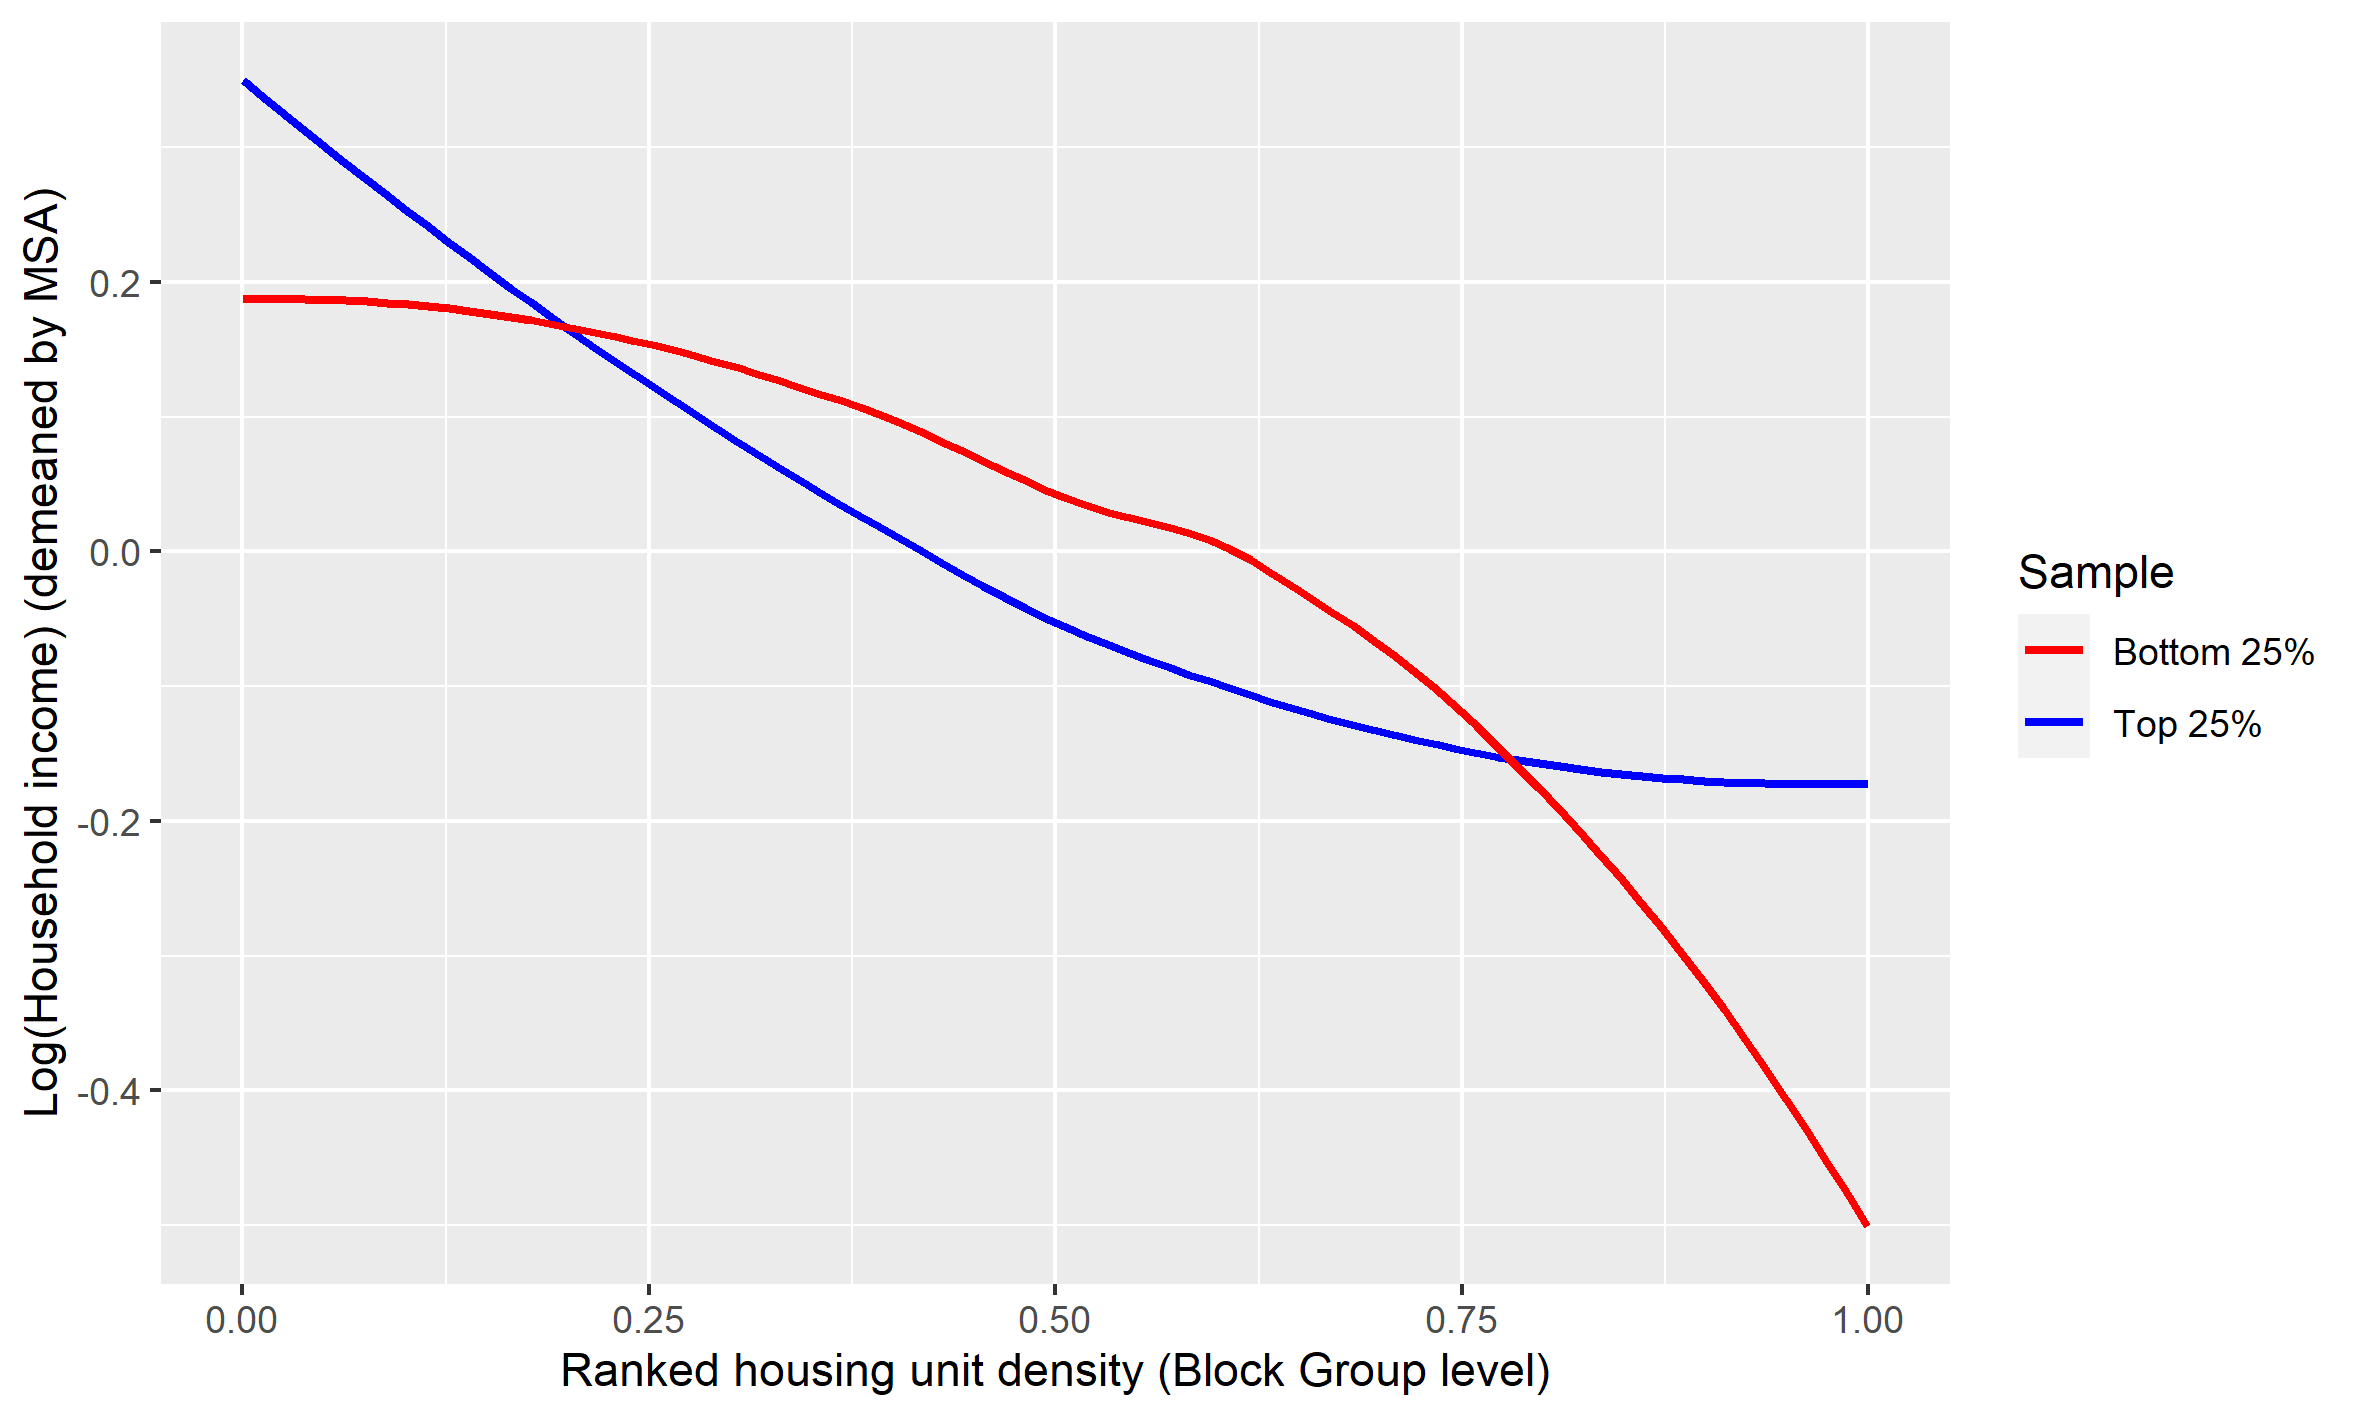
\includegraphics[width=\textwidth]{Income_dist_ctfcl.png}
			\hyperlink{Fact1}{\beamerbutton{Return}} 
\end{frame}

\begin{frame}{Conclusion}
	\begin{itemize}
		\color{black}
		\itemsep1em
		\item I show that minimum lot sizes have important implications for the macroeconomics of housing regulation
		\begin{itemize}
			\item Build and calibrate a structural GE model emphasizing both within and across city mobility
			
			\item and this mobility shapes the pattern of neighborhood amenities
		\end{itemize}
		
		\item I find substantial welfare gains of deregulation for renters across all income groups
		
		\item \dots and large losses accruing \color{red} only \color{black} to landowners in regulated neighborhoods
		\begin{itemize}
			\item corroborating reduced form evidence
		\end{itemize}
		
		\item The welfare gains appear to operate because of movement \textit{within} cities
		\begin{itemize}
			\item But residential segregation may (ironically) increase
		\end{itemize}
	\end{itemize}
\end{frame}

\bibliography{references.bib}

\section{Appendix}
\begin{frame}{Appendix: Zoning Districts}\label{zoning}
		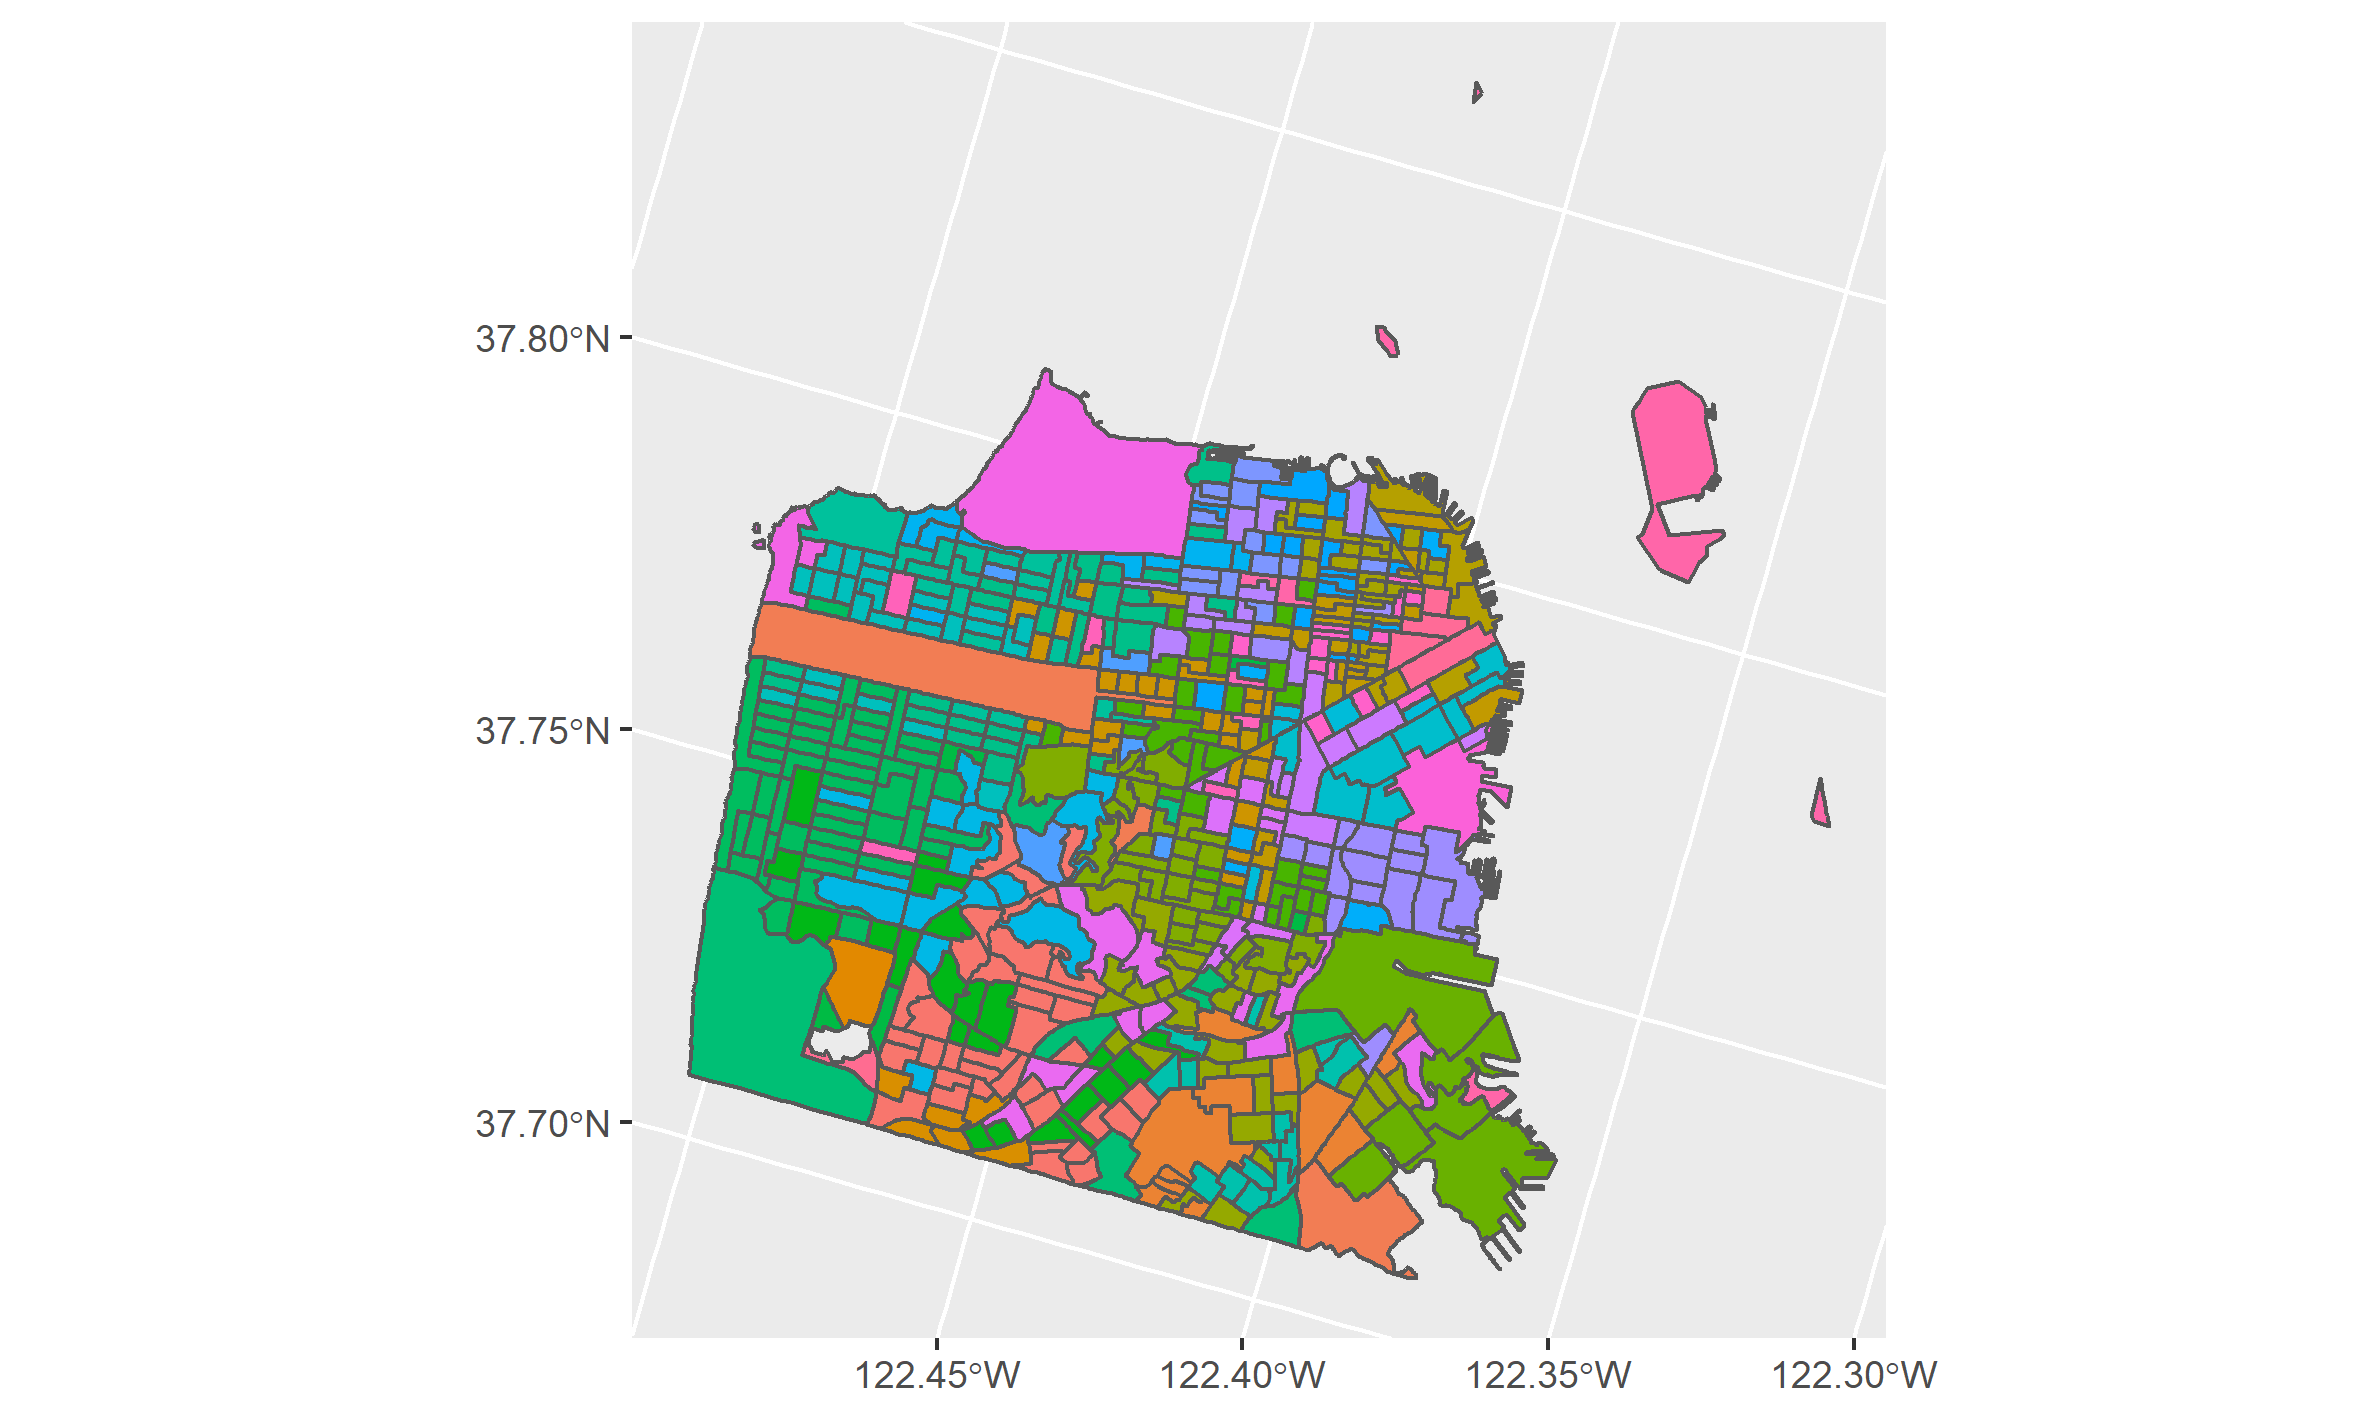
\includegraphics[width = \textwidth]{SF_MAP.png}
		\hyperlink{returnZoningDist}{\beamerbutton{Return}} 
\end{frame}

\begin{frame}{Appendix: Minimum Lot Sizes} \label{lotsizecdf}
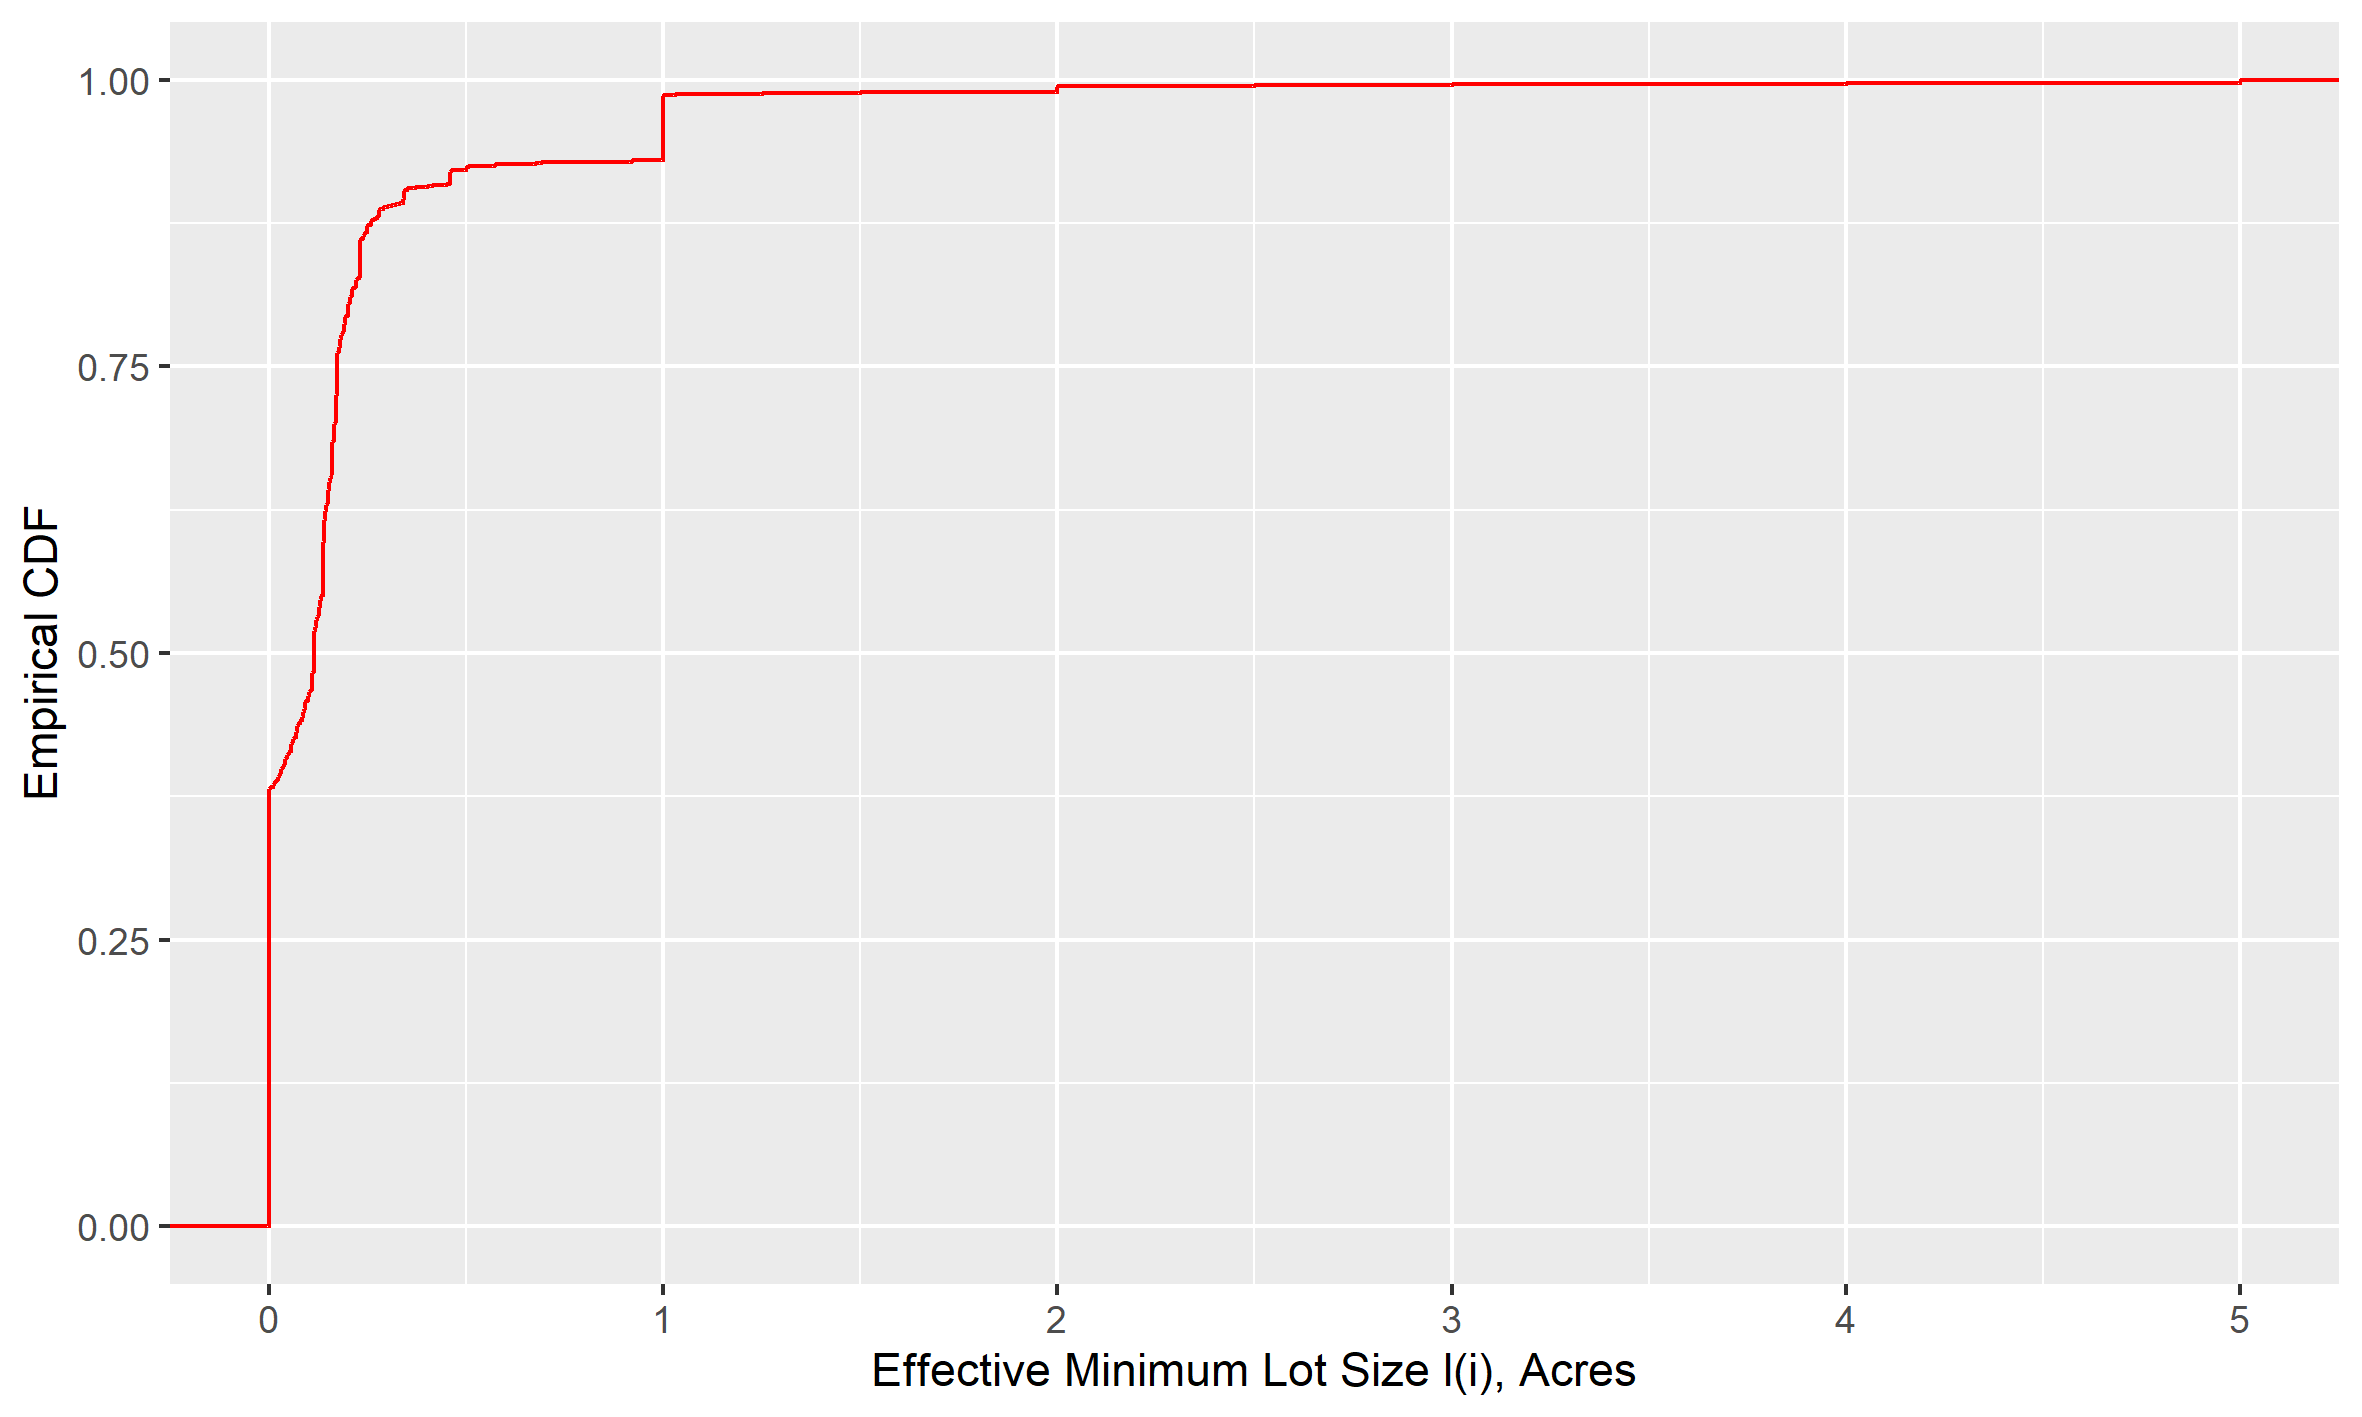
\includegraphics[width = \textwidth]{ECDFDensRegulation.png}
\end{frame}

\begin{frame}{Appendix: Minimum Lot Sizes}\label{SF_lotsize}
	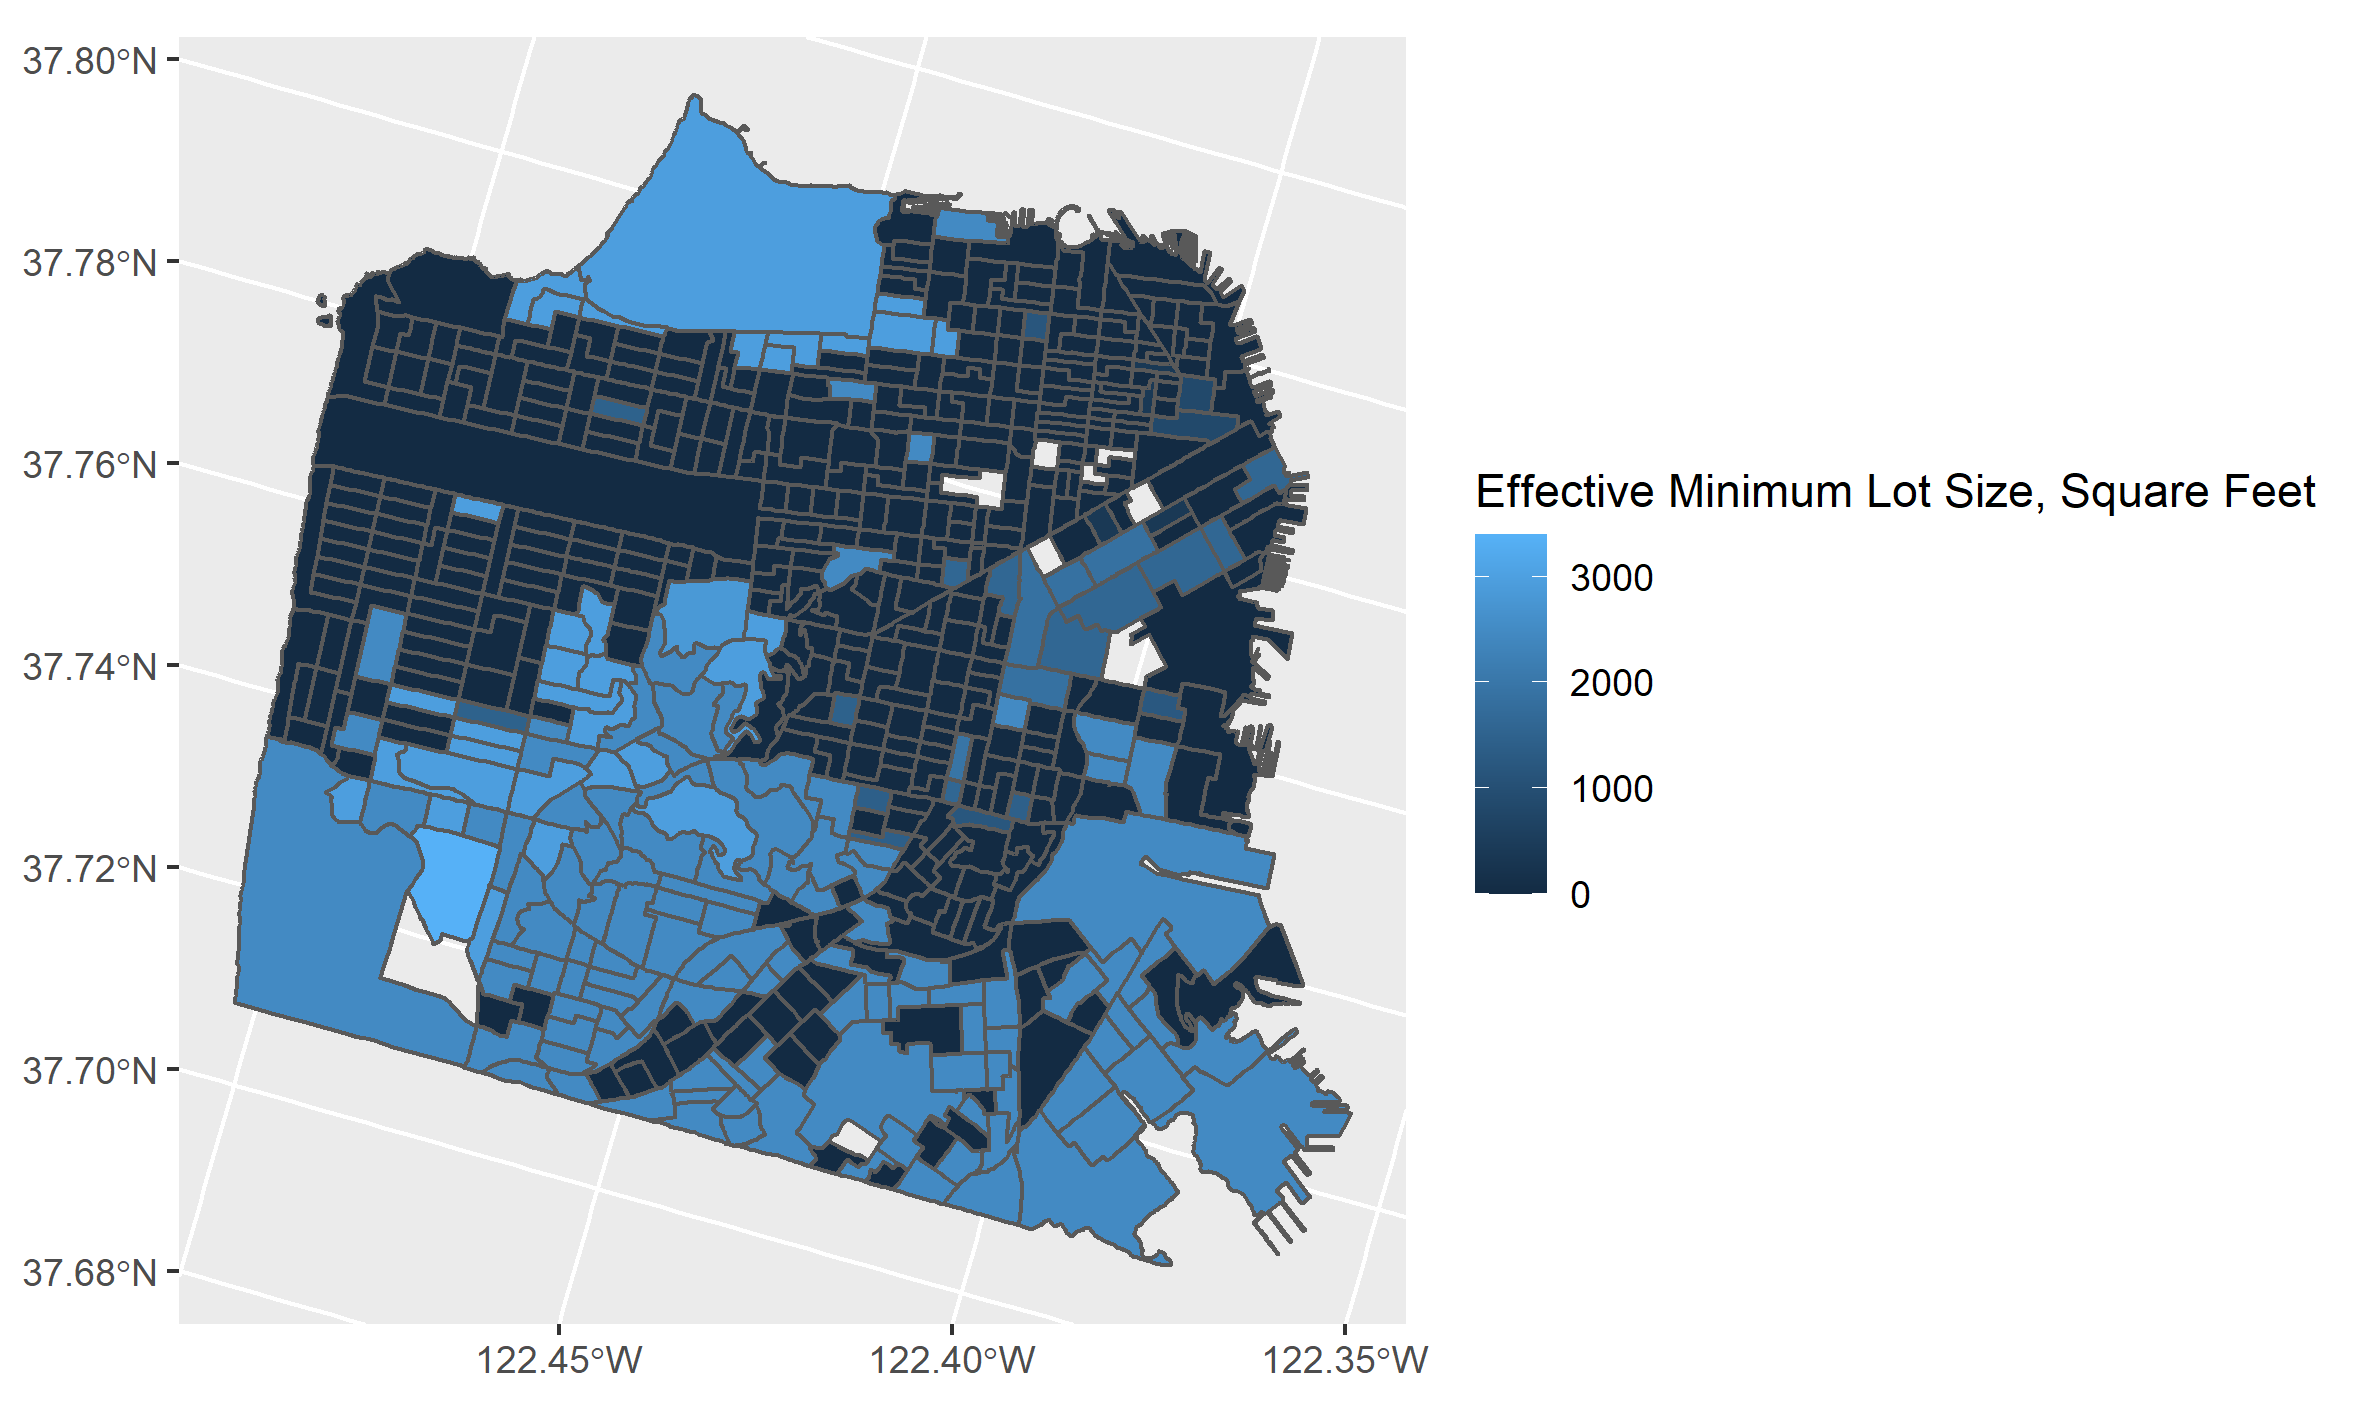
\includegraphics[width = \textwidth]{SF_EFFMINLOTSIZE.png}
	\hyperlink{returnLotSize}{\beamerbutton{Return}} 
\end{frame}


\begin{frame}{A framework for why income segregation intensifies}\label{intuition}

	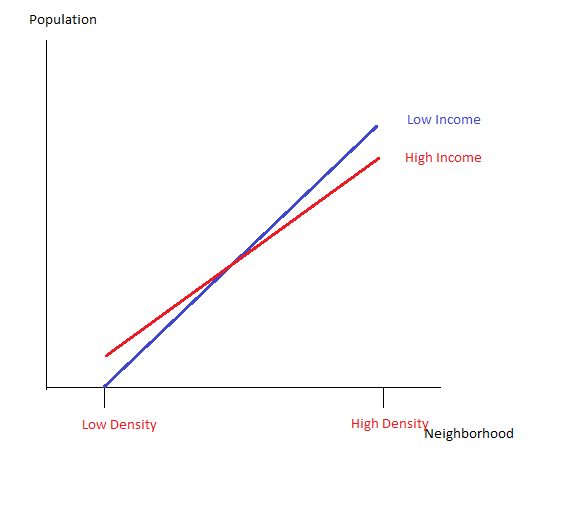
\includegraphics[width = 0.8\textwidth]{RegulatedEx.png}
	
\end{frame}

\begin{frame}{A framework for why income segregation intensifies}
	
	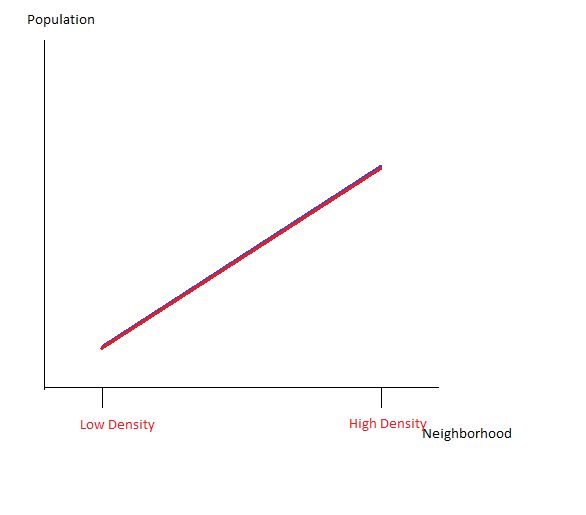
\includegraphics[width = 0.8\textwidth]{NoSorting.png}
	
	\hyperlink{returnWelfare}{\beamerbutton{Return}} 
\end{frame}

\end{document}
